%% For double-blind review submission, w/o CCS and ACM Reference (max submission space)
%\documentclass[acmsmall,review,anonymous,nonacm]{acmart}\settopmatter{printfolios=true,printccs=false,printacmref=false}
\documentclass[sigplan,10pt,review,anonymous]{acmart}\settopmatter{printfolios=true,printccs=false,printacmref=false}
%% For double-blind review submission, w/ CCS and ACM Reference
%\documentclass[acmsmall,review,anonymous]{acmart}\settopmatter{printfolios=true}
%% For single-blind review submission, w/o CCS and ACM Reference (max submission space)
%\documentclass[acmsmall,review]{acmart}\settopmatter{printfolios=true,printccs=false,printacmref=false}
%% For single-blind review submission, w/ CCS and ACM Reference
%\documentclass[acmsmall,review]{acmart}\settopmatter{printfolios=true}
%% For final camera-ready submission, w/ required CCS and ACM Reference
%\documentclass[acmsmall]{acmart}\settopmatter{}


%% Journal information
%% Supplied to authors by publisher for camera-ready submission;
%% use defaults for review submission.
\acmJournal{PACMPL}
\acmVolume{1}
\acmNumber{POPL} % CONF = POPL or ICFP or OOPSLA
\acmArticle{1}
\acmYear{2021}
\acmMonth{1}
\acmDOI{} % \acmDOI{10.1145/nnnnnnn.nnnnnnn}
\startPage{1}

%% Copyright information
%% Supplied to authors (based on authors' rights management selection;
%% see authors.acm.org) by publisher for camera-ready submission;
%% use 'none' for review submission.
\setcopyright{none}
%\setcopyright{acmcopyright}
%\setcopyright{acmlicensed}
%\setcopyright{rightsretained}
%\copyrightyear{2018}           %% If different from \acmYear

\bibliographystyle{ACM-Reference-Format}
%\citestyle{acmauthoryear}
\citestyle{acmnumeric}

%%%%%%%%

\renewcommand{\topfraction}{1} % Allow floats to take up the page
\renewcommand{\textfraction}{0}

%%%%%%%%
% \autoref from hyperref
\renewcommand{\AMSautorefname}          {Equation}
\renewcommand{\appendixautorefname}     {Appendix}
\renewcommand{\chapterautorefname}      {Chapter}
\renewcommand{\equationautorefname}     {Equation}
\renewcommand{\FancyVerbLineautorefname}{Line}
\renewcommand{\figureautorefname}       {Figure}
\renewcommand{\footnoteautorefname}     {Footnote}
\renewcommand{\Hfootnoteautorefname}    {Footnote}
\renewcommand{\itemautorefname}         {Item}
\renewcommand{\Itemautorefname}         {Item}
\renewcommand{\pageautorefname}         {Page}
\renewcommand{\paragraphautorefname}    {Section}
\renewcommand{\partautorefname}         {Part}
\renewcommand{\sectionautorefname}      {Section}
\renewcommand{\subparagraphautorefname} {Section}
\renewcommand{\subsectionautorefname}   {Section}
\renewcommand{\subsubsectionautorefname}{Section}
\renewcommand{\tableautorefname}        {Table}
\renewcommand{\theoremautorefname}      {Theorem}

%% Packages
\usepackage{booktabs}
\usepackage[rule=false]{subcaption}
\usepackage{graphicx}
\usepackage{semantic}
\let\colonapprox\undefined % Avoid redefinition error in `colonequals`
\let\colonsim\undefined % Avoid redefinition error in `colonequals`
\usepackage{colonequals}
\usepackage{mathpartir}
\usepackage{stmaryrd}
\usepackage{fontawesome}
\usepackage{array}
\usepackage{todonotes}

% \selectcolormodel{gray}

% math ligatures
\mathlig{::=}{\coloncolonequals}
\mathlig{|-}{\vdash}
\mathlig{:->}{\mapsto}
\mathlig{-->a}{\overset{a}{\longrightarrow}}
\newcommand{\abs}[1]{\left|{#1}\right|}

\def\_{\texttt{\textunderscore}}

\newcommand{\conflict}[2]{\llparenthesis#1|#2\rrparenthesis}


%%%%%%%%
% TikZ Stuff
%\usepackage{etex} % Fix "No room for new \dimen" error
\usepackage{shellesc} % Fix bug that breaks the tikz 'external' library
\usepackage{tikz}
\usetikzlibrary{babel} % Ensure compatibility the 'babel' package

\usetikzlibrary{external} % Needs to be separately enabled
%\tikzexternalize % Enable externalization
%\usepackage{lua-visual-debug}

\usetikzlibrary{arrows.meta} % Arrow Tips
\tikzset{>=Stealth}
%\tikzset{<=stealth}
%\tikzset{arrows={-Stealth[scale=50]}}
%\tikzset{edge from parent/.style={draw,->,line width=0.6pt}}
%\tikzset{wideline/.style={line width=0.7pt}}
%\tikzset{boldline/.style={color=black,line width=1.0pt}}

\usetikzlibrary{
  backgrounds,  % Provides "framed" and "gridded"
  bending,      % bending arrow tips
  decorations.pathmorphing,   % Provides wavy edges
  graphs,       % Graph *notation*
  graphdrawing, % Graph *layout*
  quotes,       % Quote syntax (e.g., "foo")
}

\usegdlibrary{
  trees,
}

\tikzset{
  %every picture/.style={framed, background rectangle/.style={draw=gray!50}},
}
\tikzset{edge style/.style={
  draw,
  %color=gray,
  font={\small\ttfamily},
  /tikz/every edge quotes/.style={
    %draw=gray!20,
    anchor=west,
    swap/.append code={
      \ifpgfarrowswap
        \pgfkeysalso{anchor=west}
      \else
        \pgfkeysalso{anchor=east}
      \fi}},
}}
\tikzset{graphs/graph style/.style={
  tree layout,
  level distance=0.5cm,
  level sep=0.5cm,
  sibling distance=0.5cm,
  sibling sep=0.1cm,
  part distance=0.1cm,
  part sep=0.1cm,
  component distance=0.1cm,
  component sep=0.1cm,
  nodes={
    draw,
    %color=gray,
    inner sep=2pt,
    rounded corners=1mm},
  edges={edge style},
}}
\tikzset{graphs/root style/.style={
 %draw=none,
 as={\textbullet$_{0}$}
}}
\tikzset{alice/.style={
  color=red!80!black,
  font={\bfseries\small},
  thick,
}}
\tikzset{bob/.style={
  color=green!60!black,
  font={\bfseries\small},
  thick,
}}
\tikzset{merge/.style={
  color=blue,
  font={\bfseries\small},
  thick,
}}
\tikzset{alice edge/.style={alice, edge style, font={\bfseries\small}}}
\tikzset{alice node/.style={alice}}
\tikzset{alice step/.style={alice}}
\tikzset{bob edge/.style={bob, edge style}, font={\bfseries\small}}
\tikzset{bob node/.style={bob}}
\tikzset{bob step/.style={bob}}
\tikzset{merge edge/.style={merge, edge style}, font={\bfseries\small}}
\tikzset{merge node/.style={merge}}
\tikzset{merge step/.style={merge,decorate,decoration={coil,amplitude=1.0pt,segment length=7.0pt,aspect=0}}}
\tikzset{star/.style={edge node={node[inner sep=0pt,at end,sloped] {\textbf{\huge${}^{*}$}}}}}

%%%%%%%%
% Lang components

% sets
\def\A{\mathcal{A}}
%\def\C{\mathcal{C}}
\def\E{\mathcal{E}}
\def\G{\mathcal{G}}
\def\I{\mathcal{I}}
\def\K{\mathcal{K}}
\def\P{\mathcal{P}}
\def\U{\mathcal{U}}
\def\V{\mathcal{V}}
\def\e{\varepsilon}
\def\AA{\textbf{A}}
\def\EE{\textbf{E}}

% constructors
\def\ExpVar{\mathsf{Exp\_var}}
\def\ExpLam{\mathsf{Exp\_lam}}
\def\ExpApp{\mathsf{Exp\_app}}
\def\ExpNum{\mathsf{Exp\_num}}
\def\ExpPlus{\mathsf{Exp\_plus}}
\def\PatVar{\mathsf{Pat\_var}}
\def\TypNum{\mathsf{Typ\_num}}
\def\TypArrow{\mathsf{Typ\_arrow}}

% indexes
\def\Root{\mathsf{Root}}
\def\LamParam{\mathsf{Lam\_param}}
\def\LamType{\mathsf{Lam\_type}}
\def\LamBody{\mathsf{Lam\_body}}
\def\AppFun{\mathsf{App\_fun}}
\def\AppArg{\mathsf{App\_arg}}
\def\PlusLeft{\mathsf{Plus\_left}}
\def\PlusRight{\mathsf{Plus\_right}}
\def\ArrowArg{\mathsf{Arrow\_arg}}
\def\ArrowResult{\mathsf{Arrow\_result}}

% actions
\def\Create{\text{Create}}
\def\Destroy{\text{Destroy}}
\def\Down{\text{Down}}
\def\Enqueue{\text{Enqueue}}
\def\Left{\text{Left}}
\def\Move{\text{Move}}
\def\Num{\text{Num}}
\def\Restore{\text{Restore}}
\def\Right{\text{Right}}
\def\Select{\text{Select}}
\def\Send{\text{Send}}
\def\Up{\text{Up}}

% relations
\DeclareMathOperator{\s}{\text{S}}
\DeclareMathOperator{\MP}{\text{MP}}
\DeclareMathOperator{\CC}{\text{C}}
\DeclareMathOperator{\D}{\text{D}}

\DeclareMathOperator{\arity}{\text{arity}}
\DeclareMathOperator{\childVertexes}{\text{childVertexes}}
\DeclareMathOperator{\cursorChildren}{\text{cursorChildren}}
\DeclareMathOperator{\vertexChildren}{\text{vertexChildren}}
\DeclareMathOperator{\deleted}{\text{deleted}}
\DeclareMathOperator{\dom}{\text{dom}}
\DeclareMathOperator{\edges}{\text{edges}}
\DeclareMathOperator{\known}{\text{known}}
\DeclareMathOperator{\liveEdges}{\text{liveEdges}}
\DeclareMathOperator{\liveVertexes}{\text{liveVertexes}}
\DeclareMathOperator{\multiparents}{\text{multiparents}}
\DeclareMathOperator{\orphans}{\text{orphans}}
\DeclareMathOperator{\parents}{\text{parents}}
\DeclareMathOperator{\parentVertexes}{\text{parentVertexes}}
\DeclareMathOperator{\reachable}{\text{reachable}}
\DeclareMathOperator{\seen}{\text{seen}}
\DeclareMathOperator{\unseen}{\text{unseen}}
\DeclareMathOperator{\vertexes}{\text{vertexes}}
\DeclareMathOperator{\vertex}{\text{vertex}}
\DeclareMathOperator{\publish}{\text{publish}}
\DeclareMathOperator{\leftIndex}{\text{leftIndex}}
\DeclareMathOperator{\rightIndex}{\text{rightIndex}}
\DeclareMathOperator{\downIndex}{\text{downIndex}}
\DeclareMathOperator{\defaultIndex}{\text{defaultIndex}}

% Define outline versions of + and -
\def\outlinepad{0.4pt}
\def\outlinestroke{0.4pt}
\newcommand{\Plus}{\mathord{
\begin{tikzpicture}[anchor=base, baseline]
%\node at (0,0) {+};
\path[draw, line width=\outlinestroke]
   ( 0.333em+\outlinestroke/2+\outlinepad,  0.270em+\outlinestroke/2+\outlinepad)
 --( 0.333em+\outlinestroke/2+\outlinepad,  0.229em-\outlinestroke/2-\outlinepad)
 --( 0.021em+\outlinestroke/2+\outlinepad,  0.229em-\outlinestroke/2-\outlinepad)
 --( 0.021em+\outlinestroke/2+\outlinepad, -0.084em-\outlinestroke/2-\outlinepad)
 --(-0.020em-\outlinestroke/2-\outlinepad, -0.084em-\outlinestroke/2-\outlinepad)
 --(-0.020em-\outlinestroke/2-\outlinepad,  0.229em-\outlinestroke/2-\outlinepad)
 --(-0.333em-\outlinestroke/2-\outlinepad,  0.229em-\outlinestroke/2-\outlinepad)
 --(-0.333em-\outlinestroke/2-\outlinepad,  0.270em+\outlinestroke/2+\outlinepad)
 --(-0.020em-\outlinestroke/2-\outlinepad,  0.270em+\outlinestroke/2+\outlinepad)
 --(-0.020em-\outlinestroke/2-\outlinepad,  0.583em+\outlinestroke/2+\outlinepad)
 --( 0.021em+\outlinestroke/2+\outlinepad,  0.583em+\outlinestroke/2+\outlinepad)
 --( 0.021em+\outlinestroke/2+\outlinepad,  0.270em+\outlinestroke/2+\outlinepad)
 --cycle
 ;
\end{tikzpicture}
}}
\newcommand{\Minus}{\mathord{
\begin{tikzpicture}[anchor=base, baseline]
%\node at (0,0) {$-$};
\path[draw, line width=\outlinestroke]
   ( 0.306em+\outlinestroke/2+\outlinepad,  0.270em+\outlinestroke/2+\outlinepad)
 --( 0.306em+\outlinestroke/2+\outlinepad,  0.229em-\outlinestroke/2-\outlinepad)
 --(-0.306em-\outlinestroke/2-\outlinepad,  0.229em-\outlinestroke/2-\outlinepad)
 --(-0.306em-\outlinestroke/2-\outlinepad,  0.270em+\outlinestroke/2+\outlinepad)
 --cycle
 ;
\end{tikzpicture}
}}

\newcommand{\hole}{\ensuremath{\square}} %\textcolor{violet}{\llparenthesis}}\textcolor{violet}{\rrparenthesis}}

% Calling \newvertex{Foo}{bar} defines
%   \vidFoo to be a new id number, and
%   \vFoo to be \texttt{bar}\ensuremath{_{\vidFoo}}
\newcounter{NodeVertexCounter}
\newcommand{\newvertex}[2]{%
\ifodd\theNodeVertexCounter
  \addtocounter{NodeVertexCounter}{1}%
\else
  \addtocounter{NodeVertexCounter}{2}%
\fi
\expandafter\newcommand\csname vid#1\endcsname{}% This is just to check if this is a redefinition
\expandafter\global\expandafter\edef\csname vid#1\endcsname{\theNodeVertexCounter}%
\expandafter\newcommand\csname v#1\endcsname{}% This is just to check if this is a redefinition
\expandafter\gdef\csname v#1\endcsname{\texttt{#2}\ensuremath{_{\csname vid#1\endcsname}}}%
}
\newcommand{\newedge}[2]{%
\ifodd\theNodeVertexCounter
  \addtocounter{NodeVertexCounter}{2}%
\else
  \addtocounter{NodeVertexCounter}{1}%
\fi
\expandafter\newcommand\csname eid#1\endcsname{}% This is just to check if this is a redefinition
\expandafter\global\expandafter\edef\csname eid#1\endcsname{\theNodeVertexCounter}%
\expandafter\newcommand\csname e#1\endcsname{}% This is just to check if this is a redefinition
\expandafter\gdef\csname e#1\endcsname{\texttt{#2}\ensuremath{_{\csname eid#1\endcsname}}}%
}
\setcounter{NodeVertexCounter}{-1}
\newvertex{Root}{Root}

% Support \includegraphics of .dot files
\DeclareGraphicsRule{.dot}{pdf}{.pdf}{`dot -Tpdf #1 -o \noexpand\OutputFile}

\newcommand{\Edge}[1]{Edge~#1}
\newcommand{\Vertex}[1]{Vertex~#1}

%%%%%%%%%%%%%%%%%%%%%%%%%%%%%%%%
%% \figureSimple
%%%%%%%%%%%%%%%%%%%%%%%%%%%%%%%%
\newedge{SimpleTimes}{Root}%
\newvertex{SimpleTimes}{*}%
\newedge{SimpleX}{L}%
\newvertex{SimpleX}{x}%
\newcommand{\figureSimple}{
\begin{figure}
\hfill
%%%%%%%%
\begin{subfigure}[t]{0.49\linewidth}
\centering
\caption{}
\label{fig:A simple tree with a hole-a}
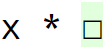
\includegraphics{code-views/simple.png}
\end{subfigure}
%%%%%%%%
\hfill
%%%%%%%%
\begin{subfigure}[t]{0.49\linewidth}
\centering
\caption{}
\label{fig:A simple tree with a hole-b}
\begin{tikzpicture}
\path (0cm,0cm) graph[graph style] {
 root[root style, color=black] -> {
  "\vSimpleTimes" [> "\eSimpleTimes", >color=black, color=black] -> {
   "\vSimpleX" [> "\eSimpleX"', >color=black, color=black],
   {}
  }
 }
};
\end{tikzpicture}
\end{subfigure}
%%%%%%%%
\hfill{}
\caption{Example of Code that Includes a Hole.
\autoref{fig:A simple tree with a hole-a}:~User Interface for the Code.
\autoref{fig:A simple tree with a hole-b}:~Graph Representation of the Code.}
\label{fig:A simple tree with a hole}
\end{figure}
}

%%%%%%%%%%%%%%%%%%%%%%%%%%%%%%%%
%% \figureConstructionAndDeletion
%%%%%%%%%%%%%%%%%%%%%%%%%%%%%%%%
\newedge{ConstructionY}{R}%
\newvertex{ConstructionY}{y}%
\newcommand{\figureConstructionAndDeletion}{
\begin{figure}
%\hfill
\hskip0.12\linewidth
%%%%%%%%
\begin{subfigure}[t]{0.43\linewidth}
\centering
\caption{
\begin{tikzpicture}[remember picture, overlay]
\path (-7.5em,0cm) node (fig-A simple tree with a hole-b-x) [gray,anchor=base west] {{\textbf{\small Fig.~\ref*{fig:A simple tree with a hole-b}}}};
%%%%
\path (0cm,0cm) node (fig-Construction) [anchor=base] {\strut};
\path [draw,->,alice step] (fig-A simple tree with a hole-b-x) to (-2em, 0cm |- fig-Construction);
\end{tikzpicture}
}
\label{fig:Construction and Deletion-a}
\label{fig:Construction}
\label{fig:Construction-b}
\begin{tikzpicture}
\path (0cm,0cm) graph[graph style] {
 root[root style] -> {
  "\vSimpleTimes" [> "\eSimpleTimes"] -> {
   "\vSimpleX" [> "\eSimpleX"'],
   "\vConstructionY" [> "\eConstructionY", >alice edge, alice node]
  }
 }
};
\end{tikzpicture}
\end{subfigure}
%%%%%%%%
\hfill
%%%%%%%%
\begin{subfigure}[t]{0.43\linewidth}
\centering
\caption{
\begin{tikzpicture}[remember picture, overlay]
\path (0cm,0cm) node (fig-Deletion) [anchor=base] {\strut};
\path [draw,->,alice step] (fig-Construction) to (-2em, 0cm |- fig-Deletion);
\end{tikzpicture}
}
\label{fig:Construction and Deletion-b}
\label{fig:Change-a}
\label{fig:Change}
\begin{tikzpicture}
\path (0cm,0cm) graph[graph style] {
 root[root style] -> {
  "\vSimpleTimes" [> "\eSimpleTimes"] -> {
   {},
   "\vConstructionY" [> "\eConstructionY"]
  }
 }
};
\path (-0.25cm,-1.7cm) graph[graph style] {
 "\vSimpleX"
};
\end{tikzpicture}
\end{subfigure}
%%%%%%%%
\hfill{}
\caption{Example of Construction and Deletion.}
\end{figure}
}

%%%%%%%%%%%%%%%%%%%%%%%%%%%%%%%%
%% \figureWrapping
%%%%%%%%%%%%%%%%%%%%%%%%%%%%%%%%
\newedge{WrapPlus}{Root}
\newvertex{WrapPlus}{+}
\newedge{WrapTimes}{L}
\newcommand{\figureWrapping}{
\begin{figure}
\hfill
%%%%%%%%
\begin{subfigure}[t]{0.32\linewidth}
\centering
\caption{
\begin{tikzpicture}[remember picture, overlay]
\path (0cm,0cm) node (fig-Wrapping-a) [anchor=base] {\strut};
\path [draw,->,alice step] (fig-Deletion) to (-2em, 0cm |- fig-Wrapping-a);
\end{tikzpicture}
}
\label{fig:Wrapping-a}
\begin{tikzpicture}
\path (0cm,0cm) graph[graph style] {
 root[root style]
};
\path (0cm,-1.7cm) graph[graph style] {
 "\vSimpleTimes" -> {
  {},
  "\vConstructionY" [> "\eConstructionY"]
 }
};
\end{tikzpicture}
\end{subfigure}
%%%%%%%%
\hfill
%%%%%%%%
\begin{subfigure}[t]{0.32\linewidth}
\centering
\caption{
\begin{tikzpicture}[remember picture, overlay]
\path (0cm,0cm) node (fig-Wrapping-b) [anchor=base] {\strut};
\path [draw,->,alice step] (fig-Wrapping-a) to (-2em, 0cm |- fig-Wrapping-b);
\end{tikzpicture}
}
\label{fig:Wrapping-b}
\begin{tikzpicture}
\path (0cm,0cm) graph[graph style] {
 root[root style] -> {
  "\vWrapPlus" [> "\eWrapPlus", >alice edge, alice node]
 }
};
\path (0cm,-1.7cm) graph[graph style] {
 "\vSimpleTimes" -> {
  {},
  "\vConstructionY" [> "\eConstructionY"]
 }
};
\end{tikzpicture}
\end{subfigure}
%%%%%%%%
\hfill
%%%%%%%%
\begin{subfigure}[t]{0.32\linewidth}
\centering
\caption{
\begin{tikzpicture}[remember picture, overlay]
\path (0cm,0cm) node (fig-Wrapping-c) [anchor=base] {\strut};
\path [draw,->,alice step] (fig-Wrapping-b) to (-2em, 0cm |- fig-Wrapping-c);
\end{tikzpicture}
}
\label{fig:Wrapping-c}
\begin{tikzpicture}
\path (0cm,0cm) graph[graph style] {
 root[root style] -> {
  "\vWrapPlus" [> "\eWrapPlus"] -> {
   "\vSimpleTimes" [> "\eWrapTimes"', >alice edge] -> {
    {},
    "\vConstructionY" [> "\eConstructionY"]
   },
   {}
  }
 }
};
\end{tikzpicture}
\end{subfigure}
%%%%%%%%
\hfill{}
\caption{Example of Wrapping.  (Note that this figure omits the orphaned \vSimpleX{} since it is no longer relevant to our narrative.)}
\label{fig:Wrapping}
\end{figure}
}

%%%%%%%%%%%%%%%%%%%%%%%%%%%%%%%%
%% \figureMovement
%%%%%%%%%%%%%%%%%%%%%%%%%%%%%%%%
\newedge{MoveTimes}{R}
\newcommand{\figureMovement}{
\begin{figure}
%\hfill
\hskip0.12\linewidth
%%%%%%%%
\begin{subfigure}[t]{0.43\linewidth}
\centering
\caption{
\begin{tikzpicture}[remember picture, overlay]
\path (-7.5em,0cm) node (fig-Wrapping-c-x) [gray,anchor=base west] {{\textbf{\small Fig.~\ref*{fig:Wrapping-c}}}};
%%%%
\path (0cm,0cm) node (fig-Moving-a) [anchor=base] {\strut};
\path [draw,->,alice step] (fig-Wrapping-c-x) to (-2em, 0cm |- fig-Moving-a);
\end{tikzpicture}
}
\label{fig:Move-a}
\begin{tikzpicture}
\path (0cm,0cm) graph[graph style] {
 root[root style] -> {
  "\vWrapPlus" [> "\eWrapPlus"]
 }
};
\path (0cm,-1.7cm) graph [graph style] {
 "\vSimpleTimes" -> {
  {},
  "\vConstructionY" [> "\eConstructionY"]
 }
};
\end{tikzpicture}
\end{subfigure}
%%%%%%%%
\hfill
%%%%%%%%
\begin{subfigure}[t]{0.43\linewidth}
\centering
\caption{
\begin{tikzpicture}[remember picture, overlay]
\path (0cm,0cm) node (fig-Moving-b) [anchor=base] {\strut};
\path [draw,->,alice step] (fig-Moving-a) to (-2em, 0cm |- fig-Moving-b);
\end{tikzpicture}
}
\label{fig:Move-b}
\begin{tikzpicture}
\path (0cm,0cm) graph[graph style] {
 root[root style] -> {
  "\vWrapPlus" [> "\eWrapPlus"] -> {
   {},
   "\vSimpleTimes" [> "\eMoveTimes", >alice edge] -> {
    {},
    "\vConstructionY" [> "\eConstructionY"]
   }
  }
 }
};
\end{tikzpicture}
\end{subfigure}
%%%%%%%%
\hfill{}
\caption{Example of Repositioning Code.}
\label{fig:Move}
\end{figure}
}

%%%%%%%%%%%%%%%%%%%%%%%%%%%%%%%%
%% \figureEditingDifferentParts
%%%%%%%%%%%%%%%%%%%%%%%%%%%%%%%%
\newedge{DifferentAlice}{L}
\newvertex{DifferentAlice}{u}
\newedge{DifferentBob}{R}
\newvertex{DifferentBob}{v}
\newcommand{\figureEditingDifferentParts}{
\begin{figure}
\hfill
%%%%%%%%
\begin{subfigure}[t]{0.32\linewidth}
\centering
\caption{
\begin{tikzpicture}[remember picture, overlay]
\path (0cm,0cm) node (fig-Editing Different Parts of the Code-a) [anchor=base] {\strut};
\path [draw,->,alice step] (fig-Moving-b) to (-2em, 0cm |- fig-Editing Different Parts of the Code-a);
\end{tikzpicture}
}
\label{fig:Editing Different Parts of the Code-a}
\begin{tikzpicture}
\path (0cm,0cm) graph[graph style] {
 root[root style] -> {
  "\vWrapPlus" [> "\eWrapPlus"] -> {
  {},
  "\vSimpleTimes" [> "\eMoveTimes"] -> {
    "\vDifferentAlice" [> "\eDifferentAlice"', >alice edge, alice node],
    "\vConstructionY" [> "\eConstructionY"]
  }
  }
 }
};
\end{tikzpicture}
\end{subfigure}
%%%%%%%%
\hfill
%%%%%%%%
\begin{subfigure}[t]{0.32\linewidth}
\centering
\caption{
\begin{tikzpicture}[remember picture, overlay]
\path (0cm,0cm) node (fig-Editing Different Parts of the Code-b) [anchor=base] {\strut};
\path [draw,->,bob step] (fig-Moving-b) to [out=15,in=165,star] (-2em, 0cm |- fig-Editing Different Parts of the Code-b);
\end{tikzpicture}
}
\label{fig:Editing Different Parts of the Code-b}
\begin{tikzpicture}
\path (0cm,0cm) graph[graph style] {
 root[root style] -> {
  "\vWrapPlus" [> "\eWrapPlus"] -> {
  {},
  "\vSimpleTimes" [> "\eMoveTimes"] -> {
    {},
    "\vDifferentBob" [> "\eDifferentBob", >bob edge, bob node]
  }
  }
 }
};
\end{tikzpicture}
\end{subfigure}
%%%%%%%%
\hfill
%%%%%%%%
\begin{subfigure}[t]{0.32\linewidth}
\centering
\caption{
\begin{tikzpicture}[remember picture, overlay]
\path (0cm,0cm) node (fig-Editing Different Parts of the Code-c) [anchor=base] {\strut};
\path [draw,->,merge step] (fig-Editing Different Parts of the Code-a) to [out=15,in=165] (-2em, 0cm |- fig-Editing Different Parts of the Code-c);
\path [draw,->,merge step] (fig-Editing Different Parts of the Code-b) to (-2em, 0cm |- fig-Editing Different Parts of the Code-c);
\end{tikzpicture}
}
\label{fig:Editing Different Parts of the Code-c}
\begin{tikzpicture}
\path (0cm,0cm) graph[graph style] {
 root[root style] -> {
  "\vWrapPlus" [> "\eWrapPlus"] -> {
  {},
  "\vSimpleTimes" [> "\eMoveTimes"] -> {
    "\vDifferentAlice" [> "\eDifferentAlice"', >merge edge, merge node],
    "\vDifferentBob" [> "\eDifferentBob", >merge edge, merge node]
  }
  }
 }
};
\end{tikzpicture}
\end{subfigure}
%%%%%%%%
\hfill{}
\caption{Example of Users Editing Different Parts of the Code.}
\label{fig:Editing Different Parts of the Code}
\end{figure}
}

%%%%%%%%%%%%%%%%%%%%%%%%%%%%%%%%
%% \figureCommutativity
%%%%%%%%%%%%%%%%%%%%%%%%%%%%%%%%
% \newcommand{\figureCommutativity}{
% \begin{figure}
% \centering
% \begin{figure}
% \centering
% \begin{tikzpicture}
% \path (-3cm, 0cm) node (a) [align=center]       {Original \\ Version};
% \path ( 0cm, 1cm) node (b) [align=center,alice node] {Alice's  \\ Version};
% \path ( 0cm,-1cm) node (c) [align=center,bob node]   {Bob's    \\ Version};
% \path ( 3cm, 0cm) node (d) [align=center]       {Combined \\ Version};
% \path [draw,->,alice step] (a) -- node [pos=0.7,auto] {Alice's Edits} (b);
% \path [draw,->,bob step]   (a) -- node [pos=0.7,auto,swap]      {Bob's Edits}   (c);
% \path [draw,->,merge step] (b) -- node [pos=0.3,auto] {Sync} (d);
% \path [draw,->,merge step] (c) -- node [pos=0.3,auto,swap]      {Sync} (d);
% \end{tikzpicture}
% \caption{TODO:Commutativity}
% \label{fig:Commutativity}
% \end{figure}
% }

%%%%%%%%%%%%%%%%%%%%%%%%%%%%%%%%
%% \figureEditingNestedParts
%%%%%%%%%%%%%%%%%%%%%%%%%%%%%%%%
\newedge{NestedAlice}{L}
\newvertex{NestedAlice}{w}
\newedge{NestedBob}{L}
\newcommand{\figureEditingNestedParts}{
\begin{figure}
%\hfill
\hskip0.12\linewidth
%%%%%%%%
\begin{subfigure}[t]{0.25\linewidth}
\centering
\caption{
\begin{tikzpicture}[remember picture, overlay]
\path (-7.5em,0cm) node (fig-Editing Different Parts of the Code-c-x) [gray,anchor=base west] {{\textbf{\small Fig.~\ref*{fig:Editing Different Parts of the Code-c}}}};
%%%%
\path (0cm,0cm) node (fig-Editing Nested Parts of the Code-a) [anchor=base] {\strut};
\path [draw,->,alice step] (fig-Editing Different Parts of the Code-c-x) to[star] (-2em, 0cm |- fig-Editing Nested Parts of the Code-a);
\end{tikzpicture}
}
\label{fig:Editing Nested Parts of the Code-a}
\begin{tikzpicture}
\path (0cm,0cm) graph[graph style] {
 root[root style] -> {
  "\vWrapPlus" [> "\eWrapPlus"] -> {
   {},
   "\vSimpleTimes" [> "\eMoveTimes"] -> {
    "\vNestedAlice" [> "\eNestedAlice"', >alice edge, alice node],
    "\vDifferentBob" [> "\eDifferentBob"]
   }
  }
 }
};
\end{tikzpicture}
\end{subfigure}
%%%%%%%%
\hfill
%%%%%%%%
\begin{subfigure}[t]{0.25\linewidth}
\centering
\caption{
\begin{tikzpicture}[remember picture, overlay]
\path (0cm,0cm) node (fig-Editing Nested Parts of the Code-b) [anchor=base] {\strut};
\path [draw,->,bob step] (fig-Editing Different Parts of the Code-c-x) to [out=15,in=165,star] (-2em, 0cm |- fig-Editing Nested Parts of the Code-b);
\end{tikzpicture}
}
\label{fig:Editing Nested Parts of the Code-b}
\begin{tikzpicture}
\path (0cm,0cm) graph[graph style] {
 root[root style] -> {
  "\vWrapPlus" [> "\eWrapPlus"] -> {
   "\vSimpleTimes" [> "\eNestedBob"', >bob edge] -> {
    "\vDifferentAlice" [> "\eDifferentAlice"'],
    "\vDifferentBob" [> "\eDifferentBob"]
   },
   {}
  }
 }
};
\end{tikzpicture}
\end{subfigure}
%%%%%%%%
\hfill
%%%%%%%%
\begin{subfigure}[t]{0.25\linewidth}
\centering
\caption{
\begin{tikzpicture}[remember picture, overlay]
\path (0cm,0cm) node (fig-Editing Nested Parts of the Code-c) [anchor=base] {\strut};
\path [draw,->,merge step] (fig-Editing Nested Parts of the Code-a) to [out=15,in=165] (-2em, 0cm |- fig-Editing Nested Parts of the Code-c);
\path [draw,->,merge step] (fig-Editing Nested Parts of the Code-b) to [out=15,in=165] (-2em, 0cm |- fig-Editing Nested Parts of the Code-c);
\end{tikzpicture}
}
\label{fig:Editing Nested Parts of the Code-c}
\label{fig:Editing Nested-c}
\begin{tikzpicture}
\path (0cm,0cm) graph[graph style] {
 root[root style] -> {
  "\vWrapPlus" [> "\eWrapPlus"] -> {
   "\vSimpleTimes" [> "\eNestedBob"', >merge edge] -> {
    "\vNestedAlice" [> "\eNestedAlice"', >merge edge, merge node],
    "\vDifferentBob" [> "\eDifferentBob"]
   },
   {}
  }
 }
};
\end{tikzpicture}
\end{subfigure}
%%%%%%%%
\hfill{}
\caption{Example of Users Editing Nested Parts of the Code.}
\label{fig:Editing Nested Parts of the Code}
\end{figure}
}

%%%%%%%%%%%%%%%%%%%%%%%%%%%%%%%%
%% \figureMultiChild
%%%%%%%%%%%%%%%%%%%%%%%%%%%%%%%%
\newedge{MultiChildAlice}{R}
\newvertex{MultiChildAlice}{x}
\newedge{MultiChildBob}{R}
\newvertex{MultiChildBob}{y}
\newcommand{\figureMultiChild}{
\begin{figure*}
%\hfill
\hskip0.12\linewidth
%%%%%%%%
\begin{subfigure}[t]{0.21\linewidth}
\centering
\caption{
\begin{tikzpicture}[remember picture, overlay]
\path (-7.5em,0cm) node (fig-Editing Nested-c-x) [gray,anchor=base west] {{\textbf{\small Fig.~\ref*{fig:Editing Nested-c}}}};
%%%%
\path (0cm,0cm) node (fig-Multi-child conflict-a) [anchor=base] {\strut};
\path [draw,->,alice step] (fig-Editing Nested-c-x) to (-2em, 0cm |- fig-Multi-child conflict-a);
\end{tikzpicture}
}
\label{fig:Multi-child-a}
\begin{tikzpicture}
\path (0cm,0cm) graph[graph style] {
 root[root style] -> {
  "\vWrapPlus" [> "\eWrapPlus"] -> {
   "\vSimpleTimes" [> "\eNestedBob"'] -> {
    "\vNestedAlice" [> "\eNestedAlice"'],
    "\vDifferentBob" [> "\eDifferentBob"]
   },
   {
    "\vMultiChildAlice" [> "\eMultiChildAlice", >alice edge, alice node]
   }
  }
 }
};
\end{tikzpicture}
\end{subfigure}
%%%%%%%%
\hfill
%%%%%%%%
\begin{subfigure}[t]{0.21\linewidth}
\centering
\caption{
\begin{tikzpicture}[remember picture, overlay]
\path (0cm,0cm) node (fig-Multi-child conflict-b) [anchor=base] {\strut};
\path [draw,->,bob step] (fig-Editing Nested-c-x) to[out=15,in=165] (-2em, 0cm |- fig-Multi-child conflict-b);
\end{tikzpicture}
}
\label{fig:Multi-child-b}
\begin{tikzpicture}
\path (0cm,0cm) graph[graph style] {
 root[root style] -> {
  "\vWrapPlus" [> "\eWrapPlus"] -> {
   "\vSimpleTimes" [> "\eNestedBob"'] -> {
    "\vNestedAlice" [> "\eNestedAlice"'],
    "\vDifferentBob" [> "\eDifferentBob"]
   },
   "\vMultiChildBob" [> "\eMultiChildBob", >bob edge, bob node]
  }
 }
};
\end{tikzpicture}
\end{subfigure}
%%%%%%%%
\hfill
%%%%%%%%
\begin{subfigure}[t]{0.21\linewidth}
\centering
\caption{
\begin{tikzpicture}[remember picture, overlay]
\path (0cm,0cm) node (fig-Multi-child conflict-c) [anchor=base] {\strut};
\path [draw,->,merge step] (fig-Multi-child conflict-a) to[out=15,in=165] (-2em, 0cm |- fig-Multi-child conflict-c);
\path [draw,->,merge step] (fig-Multi-child conflict-b) to (-2em, 0cm |- fig-Multi-child conflict-c);
\end{tikzpicture}
}
\label{fig:Multi-child-c}
\begin{tikzpicture}
\path (0cm,0cm) graph[graph style] {
 root[root style] -> {
  "\vWrapPlus" [> "\eWrapPlus"] -> {
   "\vSimpleTimes" [> "\eNestedBob"'anchor=-15] -> {
    "\vNestedAlice" [> "\eNestedAlice"'],
    "\vDifferentBob" [> "\eDifferentBob"]
   },
   "\vMultiChildAlice" [> "\eMultiChildAlice"anchor=153, >merge edge, merge node],
   {},
   "\vMultiChildBob" [> "\eMultiChildBob"anchor=195, >merge edge, merge node]
  }
 }
};
\end{tikzpicture}
\end{subfigure}
%%%%%%%%
\hfill
%%%%%%%%
\begin{subfigure}[t]{0.21\linewidth}
\centering
\caption{}
\label{fig:Multi-child-d}
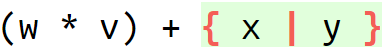
\includegraphics{code-views/multi-child-conflict.png}
\end{subfigure}
%%%%%%%%
\hfill{}
\caption{Example of Multi-Child Conflicts.}
\label{fig:Multi-child}
\end{figure*}
}

%%%%%%%%%%%%%%%%%%%%%%%%%%%%%%%%
%% \figureMultiParent
%%%%%%%%%%%%%%%%%%%%%%%%%%%%%%%%
\newedge{MultiParentAlice}{R}
\newedge{MultiParentBob}{R}
\newcommand{\figureMultiParent}{
\begin{figure*}
%\hfill
\hskip0.12\linewidth
%%%%%%%%
\begin{subfigure}[t]{0.14\linewidth}
\centering
\caption{
\begin{tikzpicture}[remember picture, overlay]
\path (-7.5em,0cm) node (fig-Multi-child-c-x) [gray,anchor=base west] {{\textbf{\small Fig.~\ref*{fig:Multi-child-c}}}};
%%%%
\path (0cm,0cm) node (fig-Multi-parent-a) [anchor=base] {\strut};
\path [draw,->,alice step] (fig-Multi-child-c-x) to[star] (-2em, 0cm |- fig-Multi-parent-a);
\end{tikzpicture}
}
\label{fig:Multi-parent-a}
\begin{tikzpicture}
\path (0cm,0cm) graph[graph style] {
 root[root style] -> {
  "\vWrapPlus" [> "\eWrapPlus"] -> {
   "\vSimpleTimes" [> "\eNestedBob"'] -> {
    "\vNestedAlice" [> "\eNestedAlice"'],
    {}
   },
   {}
  }
 }
};
\end{tikzpicture}
\end{subfigure}
%%%%%%%%
\hfill
%%%%%%%%
\begin{subfigure}[t]{0.14\linewidth}
\centering
\caption{
\begin{tikzpicture}[remember picture, overlay]
\path (0cm,0cm) node (fig-Multi-parent-b) [anchor=base] {\strut};
\path [draw,->,alice step] (fig-Multi-parent-a) to[star] (-2em, 0cm |- fig-Multi-parent-b);
\end{tikzpicture}
}
\label{fig:Multi-parent-b}
\begin{tikzpicture}
\path (0cm,0cm) graph[graph style] {
 root[root style] -> {
  "\vWrapPlus" [> "\eWrapPlus"] -> {
   "\vSimpleTimes" [> "\eNestedBob"'] -> {
    {},
    "\vNestedAlice" [> "\eMultiParentAlice"', >alice edge]
   },
   {}
  }
 }
};
\end{tikzpicture}
\end{subfigure}
%%%%%%%%
\hfill
%%%%%%%%
\begin{subfigure}[t]{0.14\linewidth}
\centering
\caption{
\begin{tikzpicture}[remember picture, overlay]
\path (0cm,0cm) node (fig-Multi-parent-c) [anchor=base] {\strut};
\path [draw,->,bob step] (fig-Multi-parent-a) to[out=15,in=165,star] (-2em, 0cm |- fig-Multi-parent-c);
\end{tikzpicture}
}
\label{fig:Multi-parent-c}
\begin{tikzpicture}
\path (0cm,0cm) graph[graph style] {
 root[root style] -> {
  "\vWrapPlus" [> "\eWrapPlus"] -> {
   "\vSimpleTimes" [> "\eNestedBob"'],
   "\vNestedAlice" [> "\eMultiParentBob", >bob edge]
  }
 }
};
\end{tikzpicture}
\end{subfigure}
%%%%%%%%
\hfill
%%%%%%%%
\begin{subfigure}[t]{0.14\linewidth}
\centering
\caption{
\begin{tikzpicture}[remember picture, overlay]
\path (0cm,0cm) node (fig-Multi-parent-d) [anchor=base] {\strut};
\path [draw,->,merge step] (fig-Multi-parent-b) to[out=15,in=165] (-2em, 0cm |- fig-Multi-parent-d);
\path [draw,->,merge step] (fig-Multi-parent-c) to[out=15,in=165] (-2em, 0cm |- fig-Multi-parent-d);
\end{tikzpicture}
}
\label{fig:Multi-parent-d}
\begin{tikzpicture}
\path (0cm,0cm) graph[graph style] {
 root[root style] -> {
  a/{\vWrapPlus} [> "\eWrapPlus"] -> {
   "\vSimpleTimes" [> "\eNestedBob"'] -> {
    {},
    b/"\vNestedAlice" [> "\eMultiParentAlice"', >merge edge]
   },
   {}
  }
 },
};
\path [draw,->,merge edge] (a) to ["\eMultiParentBob",out=-60,in=60] (b);
\end{tikzpicture}
\end{subfigure}
%%%%%%%%
\hfill
%%%%%%%%
\begin{subfigure}[t]{0.14\linewidth}
\centering
\caption{
\begin{tikzpicture}[remember picture, overlay]
\path (0cm,0cm) node (fig-Multi-parent-e) [anchor=base] {\strut};
\path [draw,->,alice step] (fig-Multi-parent-d) to (-2em, 0cm |- fig-Multi-parent-e);
\end{tikzpicture}
}
\label{fig:Multi-parent-e}
\begin{tikzpicture}
\path (0cm,0cm) graph[graph style] {
 root[root style] -> {
  v8/"\vWrapPlus" [> "\eWrapPlus"] -> {
   v2/"\vSimpleTimes" [> "\eNestedBob"'] -> {
    {},
    "\vNestedAlice" [> "\eMultiParentAlice"']
   },
   {}
  }
 }
};
\end{tikzpicture}
\end{subfigure}
%%%%%%%%
\hfill
%%%%%%%%
\begin{subfigure}[t]{0.14\linewidth}
\centering
\caption{}
\label{fig:Multi-parent-f}
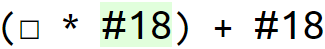
\includegraphics{code-views/multi-parent-conflict.png}
\end{subfigure}
%%%%%%%%
\hfill{}
\caption{Example of Multi-Parent Conflicts.}
\label{fig:Multi-parent}
\end{figure*}
}

%%%%%%%%%%%%%%%%%%%%%%%%%%%%%%%%
%% \figureSingleUserCycles
%%%%%%%%%%%%%%%%%%%%%%%%%%%%%%%%
% \newedge{SingleCyclePlus}{R}
% \newvertex{SingleCyclePlus}{+}
% \newedge{SingleCycleTimes}{L}
% \newvertex{SingleCycleTimes}{*}
% \newedge{SingleCycleCycle}{R}
% \newcommand{\figureSingleUserCycles}{
% \begin{figure}
% %\hfill
% \hskip0.12\linewidth
% %%%%%%%%
% \begin{subfigure}[t]{0.28\linewidth}
% \centering
% \caption{
% \begin{tikzpicture}[remember picture, overlay]
% \path (-7.5em,0cm) node (fig-Multi-parent-e-x) [gray,anchor=base west] {{\textbf{\small Fig.~\ref*{fig:Multi-parent-e}}}};
% %%%%
% \path (0cm,0cm) node (fig-Single-User Cycles-a) [anchor=base] {\strut};
% \path [draw,->,alice step] (fig-Multi-parent-e-x) to (-2em, 0cm |- fig-Single-User Cycles-a);
% \end{tikzpicture}
% }
% \label{fig:Single-User Cycles-a}
% \begin{tikzpicture}
% \path (0cm,0cm) graph[graph style] {
%  root[root style] -> {
%   v8/"\vWrapPlus" [> "\eWrapPlus"'] -> {
%   v2/"\vSimpleTimes" [> "\eNestedBob"'] -> {
%     {},
%     {}
%   },
%   {}
%   }
%  }
% };
% \end{tikzpicture}
% \end{subfigure}
% %%%%%%%%
% \hfill
% %%%%%%%%
% \begin{subfigure}[t]{0.28\linewidth}
% \centering
% \caption{
% \begin{tikzpicture}[remember picture, overlay]
% \path (0cm,0cm) node (fig-Single-User Cycles-b) [anchor=base] {\strut};
% \path [draw,->,alice step] (fig-Single-User Cycles-a) to (-2em, 0cm |- fig-Single-User Cycles-b);
% \end{tikzpicture}
% }
% \label{fig:Single-User Cycles-b}
% \begin{tikzpicture}
% \path (0cm,0cm) graph[graph style] {
%  root[root style] -> {
%   v8/"\vWrapPlus" [> "\eWrapPlus"'] -> {
%   v2/"\vSimpleTimes" [> "\eNestedBob"'] -> {
%     {},
%     "\vSingleCyclePlus" [> "\eSingleCyclePlus", >alice edge, alice node] -> {
%      "\vSingleCycleTimes" [> "\eSingleCycleTimes"', >alice edge, alice node] -> {
%       {},
%       {}
%      },
%      {}
%     }
%   },
%   }
%  }
% };
% \end{tikzpicture}
% \end{subfigure}
% %%%%%%%%
% \hfill
% %%%%%%%%
% \begin{subfigure}[t]{0.28\linewidth}
% \centering
% \caption{
% \begin{tikzpicture}[remember picture, overlay]
% \path (0cm,0cm) node (fig-Single-User Cycles-c) [anchor=base] {\strut};
% \path [draw,->,alice step] (fig-Single-User Cycles-a) to[out=15,in=165] (-2em, 0cm |- fig-Single-User Cycles-c);
% \end{tikzpicture}
% }
% \label{fig:Single-User Cycles-c}
% \begin{tikzpicture}
% \path (0cm,0cm) graph[graph style] {
%  root[root style] -> {
%   v8/"\vWrapPlus" [> "\eWrapPlus"] -> {
%   v2/"\vSimpleTimes" [> "\eNestedBob"'],
%   {}
%   }
%  }
% };
% \path[draw,->,alice edge] (v2) to ["\eSingleCycleCycle",out=-60,in=-60] (v8);
% \end{tikzpicture}
% \end{subfigure}
% %%%%%%%%
% \hfill{}
% \caption{Single-User Cycles.}
% \label{fig:Single-User Cycles}
% \end{figure}
% }

%%%%%%%%%%%%%%%%%%%%%%%%%%%%%%%%
%% \figureMultiUserCycles
%%%%%%%%%%%%%%%%%%%%%%%%%%%%%%%%
\newedge{MultiCycleTimes}{L}
\newvertex{MultiCycleTimes}{*}
\newedge{MultiCyclePlus}{R}
\newvertex{MultiCyclePlus}{+}
\newedge{MultiCycleAliceTimes}{R}
\newedge{MultiCycleAlicePlus}{L}
\newedge{MultiCycleBobPlus}{R}
\newedge{MultiCycleBobTimes}{L}
\newcommand{\figureMultiUserCycles}{
\begin{figure*}
%\hfill
\hskip0.12\linewidth
%%%%%%%%
\begin{subfigure}[t]{0.17\textwidth}
\centering
\caption{
\begin{tikzpicture}[remember picture, overlay]
\path (-7.5em,0cm) node (fig-Multi-parent-e-x) [gray,anchor=base west] {{\textbf{\small Fig.~\ref*{fig:Multi-parent-e}}}};
%%%%
\path (0cm,0cm) node (fig-Multi-User Cycles-a) [anchor=base] {\strut};
\path [draw,->,alice step] (fig-Multi-parent-e-x) to[star] (-2em, 0cm |- fig-Multi-User Cycles-a);
\end{tikzpicture}
}
\label{fig:Multi-User Cycles-a}
\begin{tikzpicture}
\path (0cm,0cm) graph[graph style] {
 root[root style] -> {
  "\vWrapPlus" [> "\eWrapPlus"] -> {
   "\vSimpleTimes" [> "\eNestedBob"'] -> {
    "\vMultiCycleTimes" [> "\eMultiCycleTimes"', >alice edge, alice node],
    "\vMultiCyclePlus" [> "\eMultiCyclePlus", >alice edge, alice node]
   },
   {}
  }
 }
};
\end{tikzpicture}
\end{subfigure}
%%%%%%%%
\hfill
%%%%%%%%
\begin{subfigure}[t]{0.17\textwidth}
\centering
\caption{
\begin{tikzpicture}[remember picture, overlay]
\path (0cm,0cm) node (fig-Multi-User Cycles-b) [anchor=base] {\strut};
\path [draw,->,alice step] (fig-Multi-User Cycles-a) to[star] (-2em, 0cm |- fig-Multi-User Cycles-b);
\end{tikzpicture}
}
\label{fig:Multi-User Cycles-b}
\begin{tikzpicture}
\path (0cm,0cm) graph[graph style] {
 root[root style] -> {
  "\vWrapPlus" [> "\eWrapPlus"] -> {
   "\vSimpleTimes" [> "\eNestedBob"'] -> {
   },
   {
    "\vMultiCycleTimes" [> "\eMultiCycleAliceTimes", >alice edge, alice node] -> {
     "\vMultiCyclePlus" [> "\eMultiCycleAlicePlus"', >alice edge, alice node],
     {}
    }
   }
  }
 }
};
\end{tikzpicture}
\end{subfigure}
%%%%%%%%
\hfill
%%%%%%%%
\begin{subfigure}[t]{0.17\textwidth}
\centering
\caption{
\begin{tikzpicture}[remember picture, overlay]
\path (0cm,0cm) node (fig-Multi-User Cycles-c) [anchor=base] {\strut};
\path [draw,->,bob step] (fig-Multi-User Cycles-a) to[out=15,in=165,star] (-2em, 0cm |- fig-Multi-User Cycles-c);
\end{tikzpicture}
}
\label{fig:Multi-User Cycles-c}
\begin{tikzpicture}
\path (0cm,0cm) graph[graph style] {
 root[root style] -> {
  "\vWrapPlus" [> "\eWrapPlus"] -> {
   "\vSimpleTimes" [> "\eNestedBob"'] -> {
   },
   {
    "\vMultiCyclePlus" [> "\eMultiCycleBobPlus", >bob edge, bob node] -> {
     "\vMultiCycleTimes" [> "\eMultiCycleBobTimes"', >bob edge, bob node],
     {}
    }
   }
  }
 }
};
\end{tikzpicture}
\end{subfigure}
%%%%%%%%
\hfill
%%%%%%%%
\begin{subfigure}[t]{0.17\textwidth}
\centering
\caption{
\begin{tikzpicture}[remember picture, overlay]
\path (0cm,0cm) node (fig-Multi-User Cycles-d) [anchor=base] {\strut};
\path [draw,->,merge step] (fig-Multi-User Cycles-b) to[out=15,in=165] (-2em, 0cm |- fig-Multi-User Cycles-d);
\path [draw,->,merge step] (fig-Multi-User Cycles-c) to (-2em, 0cm |- fig-Multi-User Cycles-d);
\end{tikzpicture}
}
\label{fig:Multi-User Cycles-d}
\begin{tikzpicture}
\path (0cm,0cm) graph[graph style] {
 root[root style] -> {
  "\vWrapPlus" [> "\eWrapPlus"] -> {
   "\vSimpleTimes" [> "\eNestedBob"'anchor=-15] -> {
   },
   v1/"\vMultiCycleTimes" [> "\eMultiCycleAliceTimes"anchor=155, >merge edge, merge node],
   {},
   v2/"\vMultiCyclePlus" [> "\eMultiCycleBobPlus"anchor=-165, >merge edge, merge node]
  }
 }
};
\path[draw,-{>[bend]},merge edge] (v1) to ["\eMultiCycleAlicePlus"anchor=south,out=-60,in=-120] (v2);
\path[draw,-{>[bend]},merge edge] (v2) to ["\eMultiCycleBobTimes"anchor=north,out=-90,in=-90] (v1);
\end{tikzpicture}
\end{subfigure}
%%%%%%%%
\hfill
%%%%%%%%
\begin{subfigure}[t]{0.17\linewidth}
\centering
\caption{}
\label{fig:Multi-User Cycles-e}
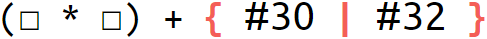
\includegraphics{code-views/cycle.png}
\end{subfigure}
%%%%%%%%
\hfill{}
\caption{Example of Cycles.}
\label{fig:Multi-User Cycles}
\end{figure*}
}

%%%%%%%%%%%%%%%%%%%%%%%%%%%%%%%%
%% \figureDisconnection
%%%%%%%%%%%%%%%%%%%%%%%%%%%%%%%%
\newedge{DisconnectionAlice}{R}
\newedge{DisconnectionBob}{L}
\newcommand{\figureDisconnection}{
\begin{figure*}
%\hfill
\hskip0.12\linewidth
%%%%%%%%
\begin{subfigure}[t]{0.17\textwidth}
\centering
\caption{
\begin{tikzpicture}[remember picture, overlay]
\path (-7.5em,0cm) node (fig-Multi-User Cycles-d-x) [gray,anchor=base west] {{\textbf{\small Fig.~\ref*{fig:Multi-User Cycles-d}}}};
%%%%
\path (0cm,0cm) node (fig-Disconnection-a) [anchor=base] {\strut};
\path [draw,->,alice step] (fig-Multi-User Cycles-d-x) to[star] (-2em, 0cm |- fig-Disconnection-a);
\end{tikzpicture}
}
\label{fig:Disconnection-a}
\begin{tikzpicture}
\path (0cm,0cm) graph[graph style] {
 root[root style] -> {
  "\vWrapPlus" [> "\eWrapPlus"] -> {
   "\vSimpleTimes" [> "\eNestedBob"'],
   "\vMultiCycleTimes" [> "\eMultiCycleAliceTimes"]
  }
 }
};
\end{tikzpicture}
\end{subfigure}
%%%%%%%%
\hfill
%%%%%%%%
\begin{subfigure}[t]{0.17\textwidth}
\centering
\caption{
\begin{tikzpicture}[remember picture, overlay]
\path (0cm,0cm) node (fig-Disconnection-b) [anchor=base] {\strut};
\path [draw,->,alice step] (fig-Disconnection-a) to[star] (-2em, 0cm |- fig-Disconnection-b);
\end{tikzpicture}
}
\label{fig:Disconnection-b}
\begin{tikzpicture}
\path (0cm,0cm) graph[graph style] {
 root[root style] -> {
  "\vWrapPlus" [> "\eWrapPlus"] -> {
   "\vSimpleTimes" [> "\eNestedBob"'] -> {
    {},
    "\vMultiCycleTimes" [> "\eDisconnectionAlice", >alice edge]
   },
   {}
  }
 }
};
\end{tikzpicture}
\end{subfigure}
%%%%%%%%
\hfill
%%%%%%%%
\begin{subfigure}[t]{0.17\textwidth}
\centering
\caption{
\begin{tikzpicture}[remember picture, overlay]
\path (0cm,0cm) node (fig-Disconnection-c) [anchor=base] {\strut};
\path [draw,->,bob step] (fig-Disconnection-a) to[out=15,in=165,star] (-2em, 0cm |- fig-Disconnection-c);
\end{tikzpicture}
}
\label{fig:Disconnection-c}
\begin{tikzpicture}
\path (0cm,0cm) graph[graph style] {
 root[root style] -> {
  "\vWrapPlus" [> "\eWrapPlus"] -> {
   {},
   "\vMultiCycleTimes" [> "\eMultiCycleAliceTimes"] -> {
    "\vSimpleTimes" [> "\eDisconnectionBob"', >bob edge],
    {}
   }
  }
 }
};
\end{tikzpicture}
\end{subfigure}
%%%%%%%%
\hfill
%%%%%%%%
\begin{subfigure}[t]{0.17\textwidth}
\centering
\caption{
\begin{tikzpicture}[remember picture, overlay]
\path (0cm,0cm) node (fig-Disconnection-d) [anchor=base] {\strut};
\path [draw,->,merge step] (fig-Disconnection-b) to[out=15,in=165] (-2em, 0cm |- fig-Disconnection-d);
\path [draw,->,merge step] (fig-Disconnection-c) to (-2em, 0cm |- fig-Disconnection-d);
\end{tikzpicture}
}
\label{fig:Disconnection-d}
\begin{tikzpicture}
\path (0cm,0cm) graph[graph style] {
 root[root style] -> {
  "\vWrapPlus" [> "\eWrapPlus"]
 }
};
\path (-0.5cm,-2cm) graph[graph style] { plus/"\vSimpleTimes" };
\path ( 0.5cm,-2cm) graph[graph style] { times/"\vMultiCycleTimes" };
\path[draw,->,merge edge] (times) to ["\eMultiCycleBobTimes"'anchor=north,out=-135,in=-45] (plus);
\path[draw,->,merge edge] (plus) to ["\eMultiCycleBobPlus"anchor=south,out=45,in=135] (times);
\end{tikzpicture}
\end{subfigure}
%%%%%%%%
\hfill
%%%%%%%%
\begin{subfigure}[t]{0.17\linewidth}
\centering
\caption{}
\label{fig:Disconnection-e}
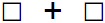
\includegraphics{code-views/disconnected-reachable.png}
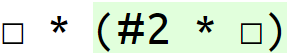
\includegraphics{code-views/disconnected-unreachable.png}
\end{subfigure}
%%%%%%%%
\hfill{}
\caption{Example of Disconnection.}
\label{fig:Disconnection}
\end{figure*}
}

\begin{document}

%% Title information
% \title[Grove]{Convergent Collaborative Structure Editing}
\title[Grove]{Grove: A Convergent Collaborative Structure-Editor Calculus}
%\subtitle{Subtitle}

%% Author information
\author{Michael D. Adams}
\orcid{0000-0003-3160-6972}

\author{Eric Griffis}
\orcid{0000-0003-1693-6172}

\author{Cyrus Omar}
\orcid{0000-0003-4502-7971}
\affiliation{
  %\position{Assistant Research Scientist}
  \department[0]{Computer Science and Engineering}
  \department[1]{Electrical Engineering and Computer Science}
  \department[2]{College of Engineering}
  \institution{University of Michigan}
  \streetaddress{Bob and Betty Beyster Building, 2260 Hayward Street}
  \city{Ann Arbor}
  \state{MI}
  \postcode{48109-2121}
  \country{USA}
}


%% Abstract
%% Note: \begin{abstract}...\end{abstract} environment must come
%% before \maketitle command
\begin{abstract}
  Text of abstract \ldots.
\end{abstract}


%% 2012 ACM Computing Classification System (CSS) concepts
%% Generate at 'http://dl.acm.org/ccs/ccs.cfm'.
%\begin{CCSXML}
%<ccs2012>
%<concept>
%<concept_id>10011007.10011006.10011008</concept_id>
%<concept_desc>Software and its engineering~General programming languages</concept_desc>
%<concept_significance>500</concept_significance>
%</concept>
%<concept>
%<concept_id>10003456.10003457.10003521.10003525</concept_id>
%<concept_desc>Social and professional topics~History of programming languages</concept_desc>
%<concept_significance>300</concept_significance>
%</concept>
%</ccs2012>
%\end{CCSXML}
%\ccsdesc[500]{Software and its engineering~General programming languages}
%\ccsdesc[300]{Social and professional topics~History of programming languages}
%% End of generated code


%% Keywords
%% comma separated list
% \keywords{keyword1, keyword2, keyword3}  %% \keywords are mandatory in final camera-ready submission


%% \maketitle
%% Note: \maketitle command must come after title commands, author
%% commands, abstract environment, Computing Classification System
%% environment and commands, and keywords command.
\maketitle


\section{Introduction}
\label{sec:Introduction}

TODO: fix the following warning which are reported by LaTeX but not Overleaf: Class acmart Warning: A possible image without description on input line 321.

Motivation:

- collaborative editing (both synchronous ala Google Docs and asynchronous version control)
is good and important as computing grows

- semantic structure editing is good because it solves the gap problem (semantic editor services
are always available) -- cite Hazelnut papers (talk about holes)

- previous approaches to collaborative editing have limitations

- diff/merge based approaches (trying to solve the inverse problem based on final states --
you lose the actual actions that were performed, and have to reconstruct them or an approx.
of them i.e. add line/delete line actions -- would need to adapt this to structure editing,
some papers have started to look at that, but fundamentally we don't want to throw away the
knowledge we have about the edits!)

- operational transforms (complexity, you have to patch previous actions based on new actions)

- CRDT-based collaborative editing (that's all been on text, not PL semantics) -- this is good
because it is relatively simple: you just send all the edits to all the replicas and they are
convergent by design

- we want to have the same convergence for a CRDT-based collaborative structure editor that maintains
the sensibility invariant of Hazelnut, i.e. every editor state has meaning. mention that maintaining sensibility
allows scaling of semantic editor services in the presence of large number of collaborators (in contrast,
using VS Code or other collaborative text editors with large numbers of collaborators means that almost always
the semantic editor services will be disabled because the program is going to be broken in multiple places
transiently)

this is tricky because:

- some edits might be conflicting -- solve this with "conflict holes"

- adding cut/paste or delete/restore allows for degenerate programs (cycles, multiple parents, etc.)

- since we are commutative, we solve both synchronus and async collaborative editing

- and this resolves issues around merges and conflicts

- contribution of this paper is to solve these problems from type-theoretic first principles:

- ...

- Hazel

\subsection{Contributions and Paper Organization}
\label{sec:Contributions and Paper Organization}

\section{Grove By Example}
\label{sec:Grove By Example}

This section introduces collaborative structure editing in Grove.
We begin in \autoref{sub:Program Representation} by covering how we use graphs to represent expressions with holes,
\autoref{sub:Single-User Actions} explores actions performed by a single user, Alice,
and \autoref{sub:Multi-user Interactions} explores actions performed by multiple users, Alice and Bob,
each of whom is editing their own instance of a program.

\subsection{Program Representation}
\label{sub:Program Representation}

\figureSimple

The \textit{program state} for each editor instance in Grove consists of a graph that represents the program being edited.
This can be presented to the user as an expression containing holes.
For example, \autoref{fig:A simple tree with a hole-b} shows one such graph,
and \autoref{fig:A simple tree with a hole-a} shows its corresponding expression,~\texttt{x * \hole}, which
has a hole on the right side of the times operator.

Program state is a directed graph with a distinguished root vertex.
%For example, \autoref{fig:A simple tree with a hole-b} shows the graph corresponding to the term in \autoref{fig:A simple tree with a hole-a}.
Each vertex represents a term and is labeled with both a globally unique identifier and a term constructor.
In \autoref{fig:A simple tree with a hole-b}, \vSimpleTimes{} and \vSimpleX{} have the constructors~\texttt{*} and \texttt{var(x)}, respectively. (For the sake of compactness, in our figures, we abbreviate \texttt{var(x)} as simply \texttt{x}.)
The root vertex has the distinguished identifier~0 and the constructor~\textbullet.

Each term constructor has an associated set of child positions.
The~\texttt{*} constructor has positions for~\texttt{L}~(i.e., left) and~\texttt{R}~(i.e., right) children
and the~\texttt{var} constructors have no child positions but takes an argument naming the particular
variable referenced~(e.g.,~\texttt{x} in \texttt{var(x)}).\footnote{Note that,
  for the purposes of this paper, we represent identifiers and number literals
  indivisibly.  See Section~TODO:REF, for how we would allow editing individual characters.}
The root vertex constructor,~\textbullet, has the single child position \texttt{Root}.

Each edge is labeled with a globally unique identifier~(e.g.,~1 and~3 in \autoref{fig:A simple tree with a hole-b}) and
a child position (e.g., \texttt{L} and \texttt{Root} in \autoref{fig:A simple tree with a hole-b}).
An edge indicates that the destination vertex is a child of the origin vertex at the given position.
%Visually, we indicate the position of an edge by the location of its origin.
For the sake of presentation clarity, we reserve odd identifiers for vertexes and even identifiers for edges.

Finally, holes are represented by the absence of a child.
For example, in \autoref{fig:A simple tree with a hole-b} the absence of a \texttt{right} edge coming from \vSimpleTimes{}
corresponds to the hole on the right of the~\texttt{*} in~\texttt{x * \hole}.

\subsection{Single-User Actions}
\label{sub:Single-User Actions}

In the remainder of this section,
we consider user actions, starting
in this subsection with single-user
actions and continuing in \autoref{sub:Multi-user Interactions}
with multi-user actions.

Each user action corresponds to one or more graph edits.
Graph edits can only add fresh edges and vertices or remove existing edges.

User actions act relative to a cursor.
We do not model cursor sharing and the cursor does not appear in the underlying graph.
We discuss cursor representations and cursor sharing in more detail in \autoref{sub:Cursors}.

\subsubsection{Construction Actions}
\label{sub:Construction}

\figureConstructionAndDeletion

To start our examples, Alice moves her cursor to the hole in~\texttt{x * \hole} in \autoref{fig:A simple tree with a hole-b}
and constructs the variable~\texttt{y} as shown in \autoref{fig:Construction-b}.
This action corresponds to creating \eConstructionY{} from \vSimpleX{} at the \texttt{R} position to a newly
created vertex, \vConstructionY{}, containing the variable reference~\texttt{y}.
The resulting graph, shown in \autoref{fig:Construction-b}, represents the expression \texttt{x * y}.

\subsubsection{Deletion Actions}
\label{sub:Deletion}

Next Alice deletes~\texttt{x} so that the code becomes~\texttt{\hole{} * y}.
This is modeled by deleting \eConstructionY{} as shown in \autoref{fig:Change-a}.
Notice that \vConstructionY{} continues to exist, and if it had any children, those children would remain connected to it.
In our system, once a vertex is created it is never deleted.
This allows further manipulations of those vertices by other users as shown later in this section.
Note that we omit such orphaned vertexes from the remaining diagrams if they are not relevant to the exposition.

Once an edge with a particular identifier is deleted, it cannot be recreated.
Thus if Alice performed an ``undo'' on this deletion, Grove would create a fresh edge between \vSimpleTimes{} and \vSimpleX{}.

\subsubsection{Wrapping Actions}
\label{sub:Wrapping}

\figureWrapping

Next, Alice types~\texttt{+} when the cursor is on \vSimpleTimes{}.
If this were a hole, this would cause a construction action to be performed as in \autoref{sub:Construction} above.
However, Alice's editor sees that this position is already occupied by the \texttt{*} expression,
so typing~\texttt{+} is interpreted as a wrapping action instead of a construction action.
This corresponds to the following sequence of graph edits, shown in \autoref{fig:Wrapping}:
(a) delete \eSimpleTimes{}, leaving \vSimpleTimes{} temporarily orphaned,
(b) add a fresh~\texttt{+} vertex (\vWrapPlus{}) as a child of the root vertex, and
(c) add an edge to \vSimpleTimes{} in the left child position of this new~\texttt{+} vertex.
(The choice of wrapping with a bias for the left child position is arbitrary.)

\subsubsection{Repositioning Actions}
\label{sub:Repositioning}

If a user wants to reposition code from one place to another, we have two options.
The first is to delete the code from its old position, and
reconstruct the code in its new position.
However, edges and vertices have unique identifiers in Grove
to support the collaborative editing features we discuss next,
so reconstruction will not preserve identity of vertices and edges.
Consequently, we take the second option: explicit repositioning actions that preserve identity.
These actions would be triggered by, for example, a drag and drop, or a cut and paste
(but not copy and paste, or a second paste after a cut, which do not need to
preserve identity and so would rely on reconstruction as already described in \autoref{sub:Construction}).

In terms of the graph, a repositioning action involves simply deleting the edge
from the original parent then adding an edge from the new parent.
Thus the code is actually \textit{repositioned}, not copied.

For example, in \autoref{fig:Move} Alice continues by
repositioning \texttt{\hole{} * y} from the left child of \texttt{+} to its right child.
This corresponds to the following sequence of graph edits, shown in \autoref{fig:Move}:
(a) delete \eWrapPlus{} leaving \vSimpleTimes{} temporarily orphaned and
(b) add \eMoveTimes{} to \vSimpleTimes{} in the right child position of \vWrapPlus{}.

\figureMovement

\subsection{Multi-user Interactions}
\label{sub:Multi-user Interactions}

Having described single-user actions,
we turn our attention to how Grove handles multiple users.
This section generalizes to any number of users,
but for simplicity we consider only two: Alice and Bob.
Alice and Bob each maintain their own editor instance and perform
actions relative to its state (using their own cursors, which we discuss in \autoref{sub:Cursors}).
We start each user where we left off in the previous section with the state shown in \autoref{fig:Move-b}.

\todo{START REV HERE}

TODO: mention that id numbers are global (or maybe use A1 and B1 for different users?)

TODO: (Place somewhere) This move semantics gives us a richer structure than
when treating code as a list of lines.  We exploit
this in Section~REF:TODO in order merge edits that involve moving code.

TODO: Common scenarios first and then consider more unusual scenarios
that cause cycles or vertices with multiple parents

\subsubsection{Editing Different Parts of the Code}
\label{sub:Editing Different Parts of the Code}

To start, Alice and Bob both have the graph in \autoref{fig:Move-b}, which
represents the code~\texttt{\hole{} + (\hole{} + y)}.

Alice adds~\vDifferentAlice{} as the left child of \vSimpleTimes{}
and Bob changes \vConstructionY{} to \vDifferentBob{}.
Before transmitting their edits to each other,
Alice and Bob have the graphs in \autoref{fig:Editing Different Parts of the Code-a}
and \autoref{fig:Editing Different Parts of the Code-b}, respectively.
(Note that thee transition edge from \autoref{fig:Move-b} to
\autoref{fig:Editing Different Parts of the Code-b} represents
multiple edges (i.e., deleting~\eConstructionY{} and adding~\eDifferentBob{} along with its child~\vDifferentBob{}).
We thus mark it with a star.)\todo{star size}\todo{"sync"}

Alice and Bob then transmit their graph edits to each other
and apply the other's graph edits to their own copy of the graph.
This results in both Alice and Bob having the graph in
\autoref{fig:Editing Different Parts of the Code-c}.

\figureEditingDifferentParts

%\figureCommutativity
\begin{figure}
  \centering
  \begin{tikzpicture}
    \path (-3cm, 0cm) node (a) [align=center]       {Original \\ Version};
    \path ( 0cm, 1cm) node (b) [align=center,alice node] {Alice's  \\ Version};
    \path ( 0cm,-1cm) node (c) [align=center,bob node]   {Bob's    \\ Version};
    \path ( 3cm, 0cm) node (d) [align=center]       {Synchronized \\ Version};
    \path [draw,->,alice step] (a) -- node [pos=0.7,auto,align=center] {Alice's \\ Edits} (b);
    \path [draw,->,bob step]   (a) -- node [pos=0.7,auto,swap,align=center]      {Bob's \\ Edits}   (c);
    \path [draw,->,merge step] (b) -- node [pos=0.3,auto] {Sync} (d);
    \path [draw,->,merge step] (c) -- node [pos=0.3,auto,swap]      {Sync} (d);
  \end{tikzpicture}
  \caption{Commutativity of Edits.}
  \label{fig:Commutativity}
\end{figure}

\subsubsection{Commutativity}
\label{sub:Commutativity}

Note that aside from transmitting edge deletions and additions,
merging requires no coordination between Alice and Bob.
For example, suppose Alice and Bob did not transmit their edits to each other
but to a third user, Chris, that has the original graph in \autoref{fig:Move-b}.
Chris can apply the edits from Alice and Bob in any order and will always get
the graph in \autoref{fig:Editing Different Parts of the Code-c}.

Stated more formally, our edit model obeys the commutativity shown in \autoref{fig:Commutativity}.
For any sequences of edits from Alice and Bob,
applying them in either order produces the same results.


\subsubsection{Editing Nested Parts of the Code}
\label{sub:Editing Nested Parts of the Code}

\figureEditingNestedParts

\figureMultiChild

After Alice and Bob share the edits they made in the previous subsection,
Alice changes~\vDifferentAlice{} to~\vNestedAlice{}, which results in the graph in \autoref{fig:Editing Nested Parts of the Code-a}.
On the other hand, Bob moves~\vSimpleTimes{} and its children from the left child of~\vWrapPlus{} to its right child
by deleting~\eMoveTimes{} and adding~\eNestedBob{}, which results in the graph in \autoref{fig:Editing Nested Parts of the Code-b}.
Since edits are based on edge identities,
both Alice's and Bob's edits can be applied to the other's graph,
which results in both Alice and Bob having the graph in \autoref{fig:Editing Nested Parts of the Code-c}.

A consequence of this design is that we allow users to modify
parts of the code that have been deleted.  For example,
Alice might receive Bob's deletion of~\eMoveTimes{} before making her
changes and before receiving Bob's addition of~\eNestedBob{}.
Her edits would then temporarily be within the code deleted by Bob.
TODO: \todo{TODO}She can restore that code using a restoration action add a fresh edge to it.

TODO:figure

Contrast with a traditional diff

Similar to how git merged across moves.
A notable difference though is that \texttt{git} detects
file moves by structural similarity rather than
our nominal equality.
(We exploit this in Subsection~REF:TODO).

\subsubsection{Multi-child conflicts}
\label{sub:Multi-child conflicts}

Next we address what happens whn edits conflict.
For example, Alice adds~\vMultiChildAlice{} as the right child of~\vWrapPlus{}
while Bob adds~\vMultiChildBob{} also as the right child of~\vWrapPlus{}.
These result in Alice and Bob having the graphs in \autoref{fig:Multi-child-a} and \autoref{fig:Multi-child-b}, respectively.
These graphs have two different edges for the~\texttt{R} position of~\vWrapPlus{}.
\autoref{fig:Multi-child-a} has~\eMultiChildAlice{}, which points to~\vMultiChildAlice{},
and \autoref{fig:Multi-child-b} has~\eMultiChildBob{}, which points to~\vMultiChildBob{}.
We call this a \emph{multi-child conflict}.

We merge these edits by including \emph{both} edges as edges going out of the \texttt{R} position
of \vWrapPlus{}.
This results in \autoref{fig:Multi-child-c}.
The conflict between Alice's and Bob's changes is
represented by the fact that there are multiple edges going out of one index.
In the user interface, we flag this conflict with the notation~\texttt{\{ x | y \}}
as shown in \autoref{fig:Multi-child-d}.

This conflict must eventually be resolved by the user by deleting
one of the edges and editing the other to be the merged value.
For example, one could delete \eMultiChildBob{} and then change~\vMultiChildAlice{}
to be~\texttt{x * y}.
(Note that users can continue to edit the code while in this conflicted state.
It just must be resolved before the the code is run.\footnote{It
  may be possible to develop evaluation models that allow these sorts of conflicts,
  but that is beyond the scope of this paper.})

TODO: need example of fully-automatic resolution and semi-automatic resolution.
Note that as a convenience to the user, certain simple
conflicts might be automatically resolved,
but we consider this a higher-level, user-interface consideration.

TODO: Multiple adds cause conflicts (Not usually presented in the UI)

Compare this to what happens when there are conflicts in a traditional,
line/diff-based version control system (e.g., \texttt{git}, \texttt{mercurial}, \texttt{svn}, etc.).
Those systems annotate files with difference markers (e.g., sequences of~\texttt{<},~\texttt{>}, or~\texttt{=})
when a merge conflict happens.
These show alternate versions of the code, and it is up to the user
to replace those alternates with the desired merged result.

Our tree-based model is similar in that it presents alternate versions
of the code, and it is up to the user to replace those alternates with the desired merged result.
Our model is different in that merge conflicts in the line-based model
prevent some semantic editor services from running
that could continue to run in the tree-based model because
code inside and outside the conflict is still valid code.
It is just the point where they meet the poses a potential problem for editor services.
Another place our model is different
is that changes are explicit rather than being inferred by a \texttt{diff} algorithm.
Finally, in our model, since all changes are in terms of
the structure of the code rather than lines,
all changes respect that structure.
This is unlike the line-based model where there is no guarantee
that a merge conflict follows the grammatical structure of the code.

\subsubsection{Multi-parent conflicts}
\label{sub:Multi-parent conflicts}

\figureMultiParent

In addition to conflicts due to multiple edges coming \emph{out of} the same child position of a particular vertex,
conflicts can manifest as multiple edges going \emph{into} a particular vertex.
We call these \emph{multi-parent conflicts}.

An example of this is shown in \autoref{fig:Multi-parent}.
\autoref{fig:Multi-parent-a} shows the graph after Alice and Bob have made some more edits,
and Alice and Bob's editors are synchronized with each other.
This graph represents the expression~\texttt{(w + \hole{}) + \hole{}}.
Alice moves~\vNestedAlice{} to the~\texttt{R} position of~\vSimpleTimes{},
while Bob moves it to the~\texttt{R} position of~\vWrapPlus{}.
This results in the graphs in \autoref{fig:Multi-parent-b} and \autoref{fig:Multi-parent-c},
which represent respectively the expression~\texttt{(\hole{} + w) + \hole{}} for Alice
and the expression~\texttt{(\hole{} + \hole{}) + w} for Bob.
In both cases, these edits are achieved with one edge delete and one edge add.
Alice deletes~\eNestedAlice{} and adds~\eMultiParentAlice{}, while
Bob deletes~\eNestedAlice{} and adds~\eMultiParentBob{}.
As explained in \autoref{sec:Formalism}, deletes are idempotent so Alice and Bob both deleting~\eNestedAlice{} is not a problem.
However, both~\eMultiParentAlice{} (added by Alice) and~\eMultiParentBob{} (added by Bob) point to the same vertex.
This generates \autoref{fig:Multi-parent-d}, in which~\vNestedAlice{} has two parents pointing to it.
We call this situation a multi-parent conflict.

TODO: talk about how to resolve the conflict

% \subsubsection{Single-User Cycles}
% \label{sub:Cycles}

% TODO: cut this section

% \figureSingleUserCycles

% Another case we must consider is when cycles appear in the graph.
% We categorize these into cycles caused by the action of a single user
% and cycles caused by the interaction of the actions of multiple users.

% In a single user context,
% normal insertion and deletion of code by the user cannot create cycles.
% However, it is possible with certain kinds of copy and paste.
% For example, suppose Alice is editing the code in \autoref{fig:Single-User Cycles-a}
% and uses copy and paste to copy \Vertex{TODO} to the right child of \Vertex{TODO}.
% There are two ways to interpret the paste action.
% The first interpretation is to create a deep copy of \Vertex{TODO}.
% This results in \autoref{fig:Single-User Cycles-b} and
% does not cause a cycle.
% The second interpretation is to simply add an edge to \Vertex{TODO}.
% This results in \autoref{fig:Single-User Cycles-b}
% and causes a cycle.

% Note that not all pastes should be deep copies.
% For example, Alice may have accomplished code move in \autoref{sub:Editing Nested Parts of the Code}
% by a cutting from the old position and pasting to the new position.
% Preserving Bob's nested edits requires that the paste be by reference instead of by copy.
% Distinguishing when a paste should be by reference versus by copy
% is ultimately a user interface question.
% Cycles caused by the local user's edits can be detected as soon as a user enters them
% by noting either that the graph would contain a cycle or the vertex
% already has a parent somewhere in the graph.

% Thus, as a user interface consideration, it might be best to either
% disallow such edits to at least warn users when their
% edits would create a cycle.

\subsubsection{Cycles}
\label{sub:Multi-User Cycles}

\figureMultiUserCycles

TODO: paragraph about why single-user cycles cannot happen.
While single-user edits can be checked to see
whether they create a cycle and thus the system
can immediately warn the user,
multi-user edits may not manifest cycles until after
the edits from multiple users are merged.

For example, consider the situation in \autoref{fig:Multi-User Cycles}.
\autoref{fig:Multi-User Cycles-a} shows the graph after Alice and Bob have made some more edits,
and Alice and Bob's editors are synchronized with each other.
This graph represents the expression~\texttt{((\hole{} + \hole{}) + (\hole{} * \hole{})) + \hole}.
Alice moves~\vMultiCycleTimes{} to the \texttt{R} child of~\vWrapPlus{}
and then~\vMultiCyclePlus{} underneath.
This results in \autoref{fig:Multi-User Cycles-b},
which represents the expression~\texttt{(\hole{} + \hole{}) + ((\hole{} * \hole{}) + \hole{})}.
On the other hand, Bob does the same
but puts~\vMultiCycleTimes{} and under~\vMultiCyclePlus{}.
This results in \autoref{fig:Multi-User Cycles-c},
which represents the expression~\texttt{(\hole{} + \hole{}) + ((\hole{} + \hole{}) * \hole{})}.

On their own, neither of these edits creates a cycle.
However, merging the edit actions of both Alice and Bob results in the graph
in \autoref{fig:Multi-User Cycles-d}, which has a cycle
between~\vMultiCycleTimes{} and~\vMultiCyclePlus{}.
This situation is akin to a merge conflict in traditional version control systems.
Resolving it requires user input, but is as simple as
either deleting~\eMultiCycleBobPlus{} and~\eMultiCycleBobTimes{}~(thus favoring Alice's version)
or deleting~\eMultiCycleAliceTimes{} and~\eMultiCycleAlicePlus{}~(thus favoring Bob's version).
Since a cycle like this that is connected to the root vertex always
contains vertexes with multiple parents that if removed would break the cycle,
we use the user interface described in \autoref{sub:Multi-parent conflicts}
to display these kinds of programs.
For example, \autoref{fig:Multi-User Cycles-d} would be displayed
as shown in \autoref{fig:Multi-User Cycles-e}.
We leave the user interface considerations of resolving the conflict such a
cycle represents to future work.


\subsubsection{Disconnection}
\label{sub:Disconnection}

\figureDisconnection

\todo{UI would show orphans only once edits orphans occur}

Finally, when multi-user edits are merged,
parts of the graph can become disconnected
even though they are connected in each user's
copy of the graph before the merge.

For example, consider the situation in \autoref{fig:Disconnection}.
\autoref{fig:Disconnection-a} shows the graph after Alice and Bob have made some more edits,
and Alice and Bob's editors are synchronized with each other.
This graph represents the expression~\texttt{(\hole{} * \hole{}) + (\hole{}  * \hole{})}.
Alice moves~\vMultiCycleTimes{} under~\vSimpleTimes{}.
This results in \autoref{fig:Disconnection-b},
which represents the expression~\texttt{(\hole{} * (\hole{} * \hole{})) + \hole}.
On the other hand, Bob puts~\vSimpleTimes{} and under~\vMultiCycleTimes{}.
This results in \autoref{fig:Disconnection-c},
which represents the expression~\texttt{\hole{} + ((\hole{} * \hole{}) * \hole{})}.

When these edits are merged, the result is the graph in \autoref{fig:Disconnection-d}.
Since Alice deleted~\eNestedBob{}
and Bob deleted~\eMultiCycleAliceTimes{},
when these are merged~\vMultiCycleTimes{} and~\vSimpleTimes{}
are disconnected from the root.

This is similar to the type of merge conflict
that can arise in traditional version control systems
when two users delete different functions that
are duplicates of the other.

Fortunately, we can detect this situation and warn the user
since the disconnection appears after merging two graphs
that did not have disconnected vertexes.

\subsection{Cursors}
\label{sub:Cursors}

Cursor is either on edge or on position

cursors are advisory

Don't model communication but would be separate layer anyway

\section{Formalism}
\label{sec:Formalism}

We will now make the intuitions developed in the previous section precise
by defining a collaborative structure editor calculus called Grove.
We begin in Sec.~\ref{sub:Syntax} with the syntax, then discuss
the internal graph representation in Sec.~\ref{sub:Convergent Graphs},
...


TODO: point of this section is commutativity theorem

TODO: (though as we show in \autoref{sec:Formalism} creating a vertex is implicit in edge creation)

The formalism is rather simple, \autoref{sec:Grove By Example} shows
that it is sufficient to handle many common situations,
and this simplicity aids in the predictability.

% $\arraycolsep=2pt\begin{array}{llcl}
% \mathsf{Typ} & \tau & ::= & t ~\vert~ \aparr{\tau}{\tau} ~\vert~ \aall{t}{\tau} ~\vert~ \arec{t}{\tau} ~\vert~ \aprod{\labelset}{\mapschema{\tau}{i}{\labelset}} ~\vert~ \asum{\labelset}{\mapschema{\tau}{i}{\labelset}}\\
% \mathsf{Exp} & e & ::= & x ~\vert~ \aelam{\tau}{x}{e} ~\vert~ \aeap{e}{e} ~\vert~ \aetlam{t}{e} ~\vert~ \aetap{e}{\tau} ~\vert~ \aefold{e} ~\vert~ \aetpl{\labelset}{\mapschema{e}{i}{\labelset}} ~\vert~  \aein{\ell}{e} \\
% & & \vert & \aematchwith{n}{e}{\seqschemaX{r}}\\
% \mathsf{Rule} & r & ::= & \aematchrule{p}{e}\\
% \mathsf{Pat} & p & ::= & x  ~\vert~ \aewildp ~\vert~ \aefoldp{p} ~\vert~ \aetplp{\labelset}{\mapschema{p}{i}{\labelset}} ~\vert~ \aeinjp{\ell}{p}
% \end{array}$

\begin{figure}
  \[
    \arraycolsep=0pt
    \begin{array}{lrlll}
      \textrm{Patterns:}          & p    & {}\in Pat & {}::={} & x \mid \_                                                            \\
      \textrm{Expressions:\qquad} & e    & {}\in Exp & {}::={} & x \mid \lambda p\mathord{:}\tau.e \mid e~e \mid e + e \mid n \mid \_ \\
      \textrm{Types:}             & \tau & {}\in Typ & {}::={} & \tau \rightarrow \tau \mid Num \mid \_                               \\
    \end{array}
  \]
  \caption{Syntax as a grammar for the lambda calculus that we are considering.}
  \label{fig:Syntax as a grammar}
\end{figure}

\subsection{Syntax}
\label{sub:Syntax}

The language we are modeling is shown in \autoref{fig:Syntax as a grammar}.
Standard for a simply-typed lambda calculus except that
all terms have holes (represented by $\_$)
and the argument to a lambda is its own term.
The latter of which allows us to express lambdas with a hole for the bound variable.

In order to model this we define


Turn that into a constructor set K + index set I + arity function (has type: K -> $\wp$(I)).


\begin{figure}
  \[
    \arraycolsep=0pt
    \begin{array}{ll}
      \arity : \K \rightarrow & \wp(\I)                                        \\
      \hline
      \arity(\Root)={}        & \left\{ \Root \right\}                         \\
      \arity(\PatVar)={}      & \left\{ \right\}                               \\
      \arity(\ExpVar)={}      & \left\{ \right\}                               \\
      \arity(\ExpLam)={}      & \left\{ \LamParam, \LamType, \LamBody \right\} \\
      \arity(\ExpApp)={}      & \left\{ \AppFun, \AppArg \right\}              \\
      \arity(\ExpPlus)={}     & \left\{ \PlusLeft, \PlusRight \right\}         \\
      \arity(\TypArrow)={}    & \left\{ \ArrowArg, \ArrowResult \right\}       \\
      \arity(\TypNum)={}      & \left\{ \right\}                               \\
    \end{array}
  \]
  \caption{Constructors, Indexes and Arity}
  \label{fig:Constructors, Indexes and Arity}
\end{figure}

\subsection{Convergent Graphs}
\label{sub:Convergent Graphs}

\subsubsection{Graphs}
\label{sub:Graphs}

TODO: rename indices to positions

TODO: look into using bold plus and minus (google results)

A graph $\G : \E \rightarrow \Sigma$ is a function from edges to edge states,
where $\E = \U \times \V \times \P \times \V$,
and   unique IDs are drawn from some suitable set $\U$,
and   vertices are drawn from $\V$,
and   positions are drawn from $\P$,
and   edge states are drawn from $\Sigma$, all defined below.

Each edge $\e = (u, v, p, v^\prime)$ has a unique name, $u \in \U$,
and connects the child position $p$ of a source vertex $v$ to a target vertex $v^\prime$.
The state of each edge, $\e$, is determined by the corresponding edge state, $\G(\e) \in \Sigma = \{ \bot, \Plus, \Minus \}$.
If $\G(\e) = \bot$, then $\e$ does not yet exist.
If $\G(\e)$ is $\Plus$, the edge has been created.
If $\G(\e)$ is $\Minus$, the edge has been destroyed.
The total ordering $\bot \sqsubset \Plus \sqsubset \Minus$ forms a lattice over $\Sigma$.

A vertex $v = (u, k)$ identifies a distinct instance of the constructor $k$.

A constructor $k \in \K$ represents a different type of node in the target language's abstract syntax tree.

A position $p \in \P$ identifies a location, adjacent to some parent vertex.

Every graph contains a distinguished root vertex, root constructor, and root position, respectively named $v_0$, $k_0$, and $p_0$.



% Define $\sqcup_{edge state}$ (i.e. join)

% lattice ordering $\bot < + < -$ LUB e.g., join A B = C

You can map from syntax to graph by selecting
unique IDs $u$ (for both edges and vertexes).
- holes are not explicit in the graph

\subsubsection{Graph Edits}
\label{sub:Graph Edits}

We define graph edit actions as a pair of an edge state, excluding $\bot$, and an edge.
Thus, $\alpha \in \A = \left\{\Plus, \Minus\right\} \times \E$.
As a shorthand, we define $+e$ to be $(\Plus, e)$ and $-e$ to be $(\Minus, e)$.

We define the join operation $s_1 \sqcup s\_2$ to be the least upper bound of $s_1$ and $s_2$ with respect to the $\sqsubset$ ordering.
For example, $\Plus \sqcup \bot = \Plus$, which means edges can be created if they have never existed,
and $\Plus \sqcup \Minus = \Minus$, which means that once an edge is deleted it can never be restored.
%smallest element of $\Sigma$ that is greater than or equal to both $s_1$ and $s_2$.

We define the semantics of graph actions via the following
transition relation between graphs.
\[
  G \overset{\left(s,e\right)}{\longrightarrow} G\left[ e \mapsto s \sqcup G(e) \right\}
\]
In other words, applying graph action $\alpha = \left(s, e\right)$ to a graph $G$
results in $G\left[e \mapsto s \sqcup G(e) \right]$ (i.e., the graph is updated at $e$ to be
the join of $s$ with whatever was already at $e$).

% Graph action semantics is a transition system between graphs.
% (join with whatever it was before)

% Intuitively, joining any edge state with $\bot$ is always the non-$\bot$ edge state (once an edge exists, it always exists).
% Joining anything with $\Minus$ is always $\Minus$ (once an edge is marked as deleted, it is permanently deleted).

\subsection{Commutativity}

In order to define commutativity, we first define a lattice over $G$.
Then we show that for any graphs $G$ and $G'$ and graph action $\alpha$,
$G \overset{\alpha}\rightarrow G'$
iff $G \sqcup \llbracket\alpha\rrbracket = G'$.
Thus the commutativity of graph actions is established
by the commutativity of the join operations defining those graph actions.

Discuss uniqueness of uuid

\begin{lemma}[Join Commutativity]
  \label{lem:Join Commutativity}
\end{lemma}

\begin{lemma}[Joining]
  \label{lem:Joining}
  For all graphs $G$ and $G'$ and all edit actions $\alpha$,
  $G \overset{\alpha}{\longrightarrow} G'$
  iff $G \sqcup \llbracket\alpha_1\rrbracket = G'$.
\end{lemma}
\begin{proof}
  If $G \overset{\alpha_1\alpha_2}{\longrightarrow} G'$
\end{proof}


\begin{theorem}[Commutativity]
  \label{thm:Commutativity}
  For all graphs $G$ and $G'$ and all edit actions $\alpha_1$ and $\alpha_2$,
  if $G \overset{\alpha_1\alpha_2}{\longrightarrow} G'$,
  then $G \overset{\alpha_2\alpha_1}{\longrightarrow} G'$.
\end{theorem}
\begin{proof}
  Using \autoref{lem:Joining} to unfold $\rightarrow$ into $\sqcup$,
  $G \sqcup \llbracket\alpha_1 \sqcup \llbracket \sqcup \alpha_2 \rrbracket = G'$.
  Then by \autoref{lem:Join Commutativity},
  $G \sqcup \llbracket\alpha_2 \sqcup \llbracket \sqcup \alpha_1 \rrbracket = G'$.
  Finally using \autoref{lem:Joining} to fold $\sqcup$ into $\rightarrow$,
  $G \overset{\alpha_2\alpha_1}{\longrightarrow} G'$.
\end{proof}

\subsubsection{Agda Mechanization}
\label{sub:Agda Mechanization}

\subsection{Graph Decomposition}
\label{sub:Graph Decomposition}

What does a graph decomposition produce? a 4-tuple (reachable, multiparented, deleted, simple cycles).

A simple cycle is a set of vertices connected by a closed path, consisting
of:

1) two or more vertices, all descendants of each other, and
2) the vertices of any non-multiparent subtrees reachable from the core, and
not reachable from the root vertex.

To determine the simple cycles of a graph, we:

1) check if any vertex in the graph is a descendant of itself or some other
vertex that is (a descendant of itself),
2) find the least vertex in the core of this new(ly discovered) cycle, and
3) return a tree connecting every vertex reachable from the least (vertex).

The least vertex of a cycle is the one that was created first. To ensure consistent behavior, the search for reachable vertices begins at the least vertex in a cycle.

<Mathematical definition of above.>

\subsection{User Actions}
\label{sub:User Actions}

Mapping to b actions

\[
  \begin{array}{l}
    \textrm{User Actions}: \grave{e} \in Act ::= e \mid \#u \mid \conflict{\grave{e}}{\grave{e}}                                                       \\
    \s : \G \to Act \times \V^{*} \times \V^{*} \times \V^{*}                                                                                          \\
    \s(G) = (\grave{e}, \MP(G), \CC(G), \D(G))                                                                                                         \\
    \MP(G) = \left\{ v \in \vertexes(G) \mid \exists e_1,e_2 \in \liveEdges(G), e_1= \right.                                                           \\
    \qquad \left. (v,p_1,v_1), e_2=(v,p_2,v_2), e_1 \ne e_2 \right\}                                                                                   \\
    \CC(G) = \ldots                                                                                                                                    \\
    \D(G) = \orphans(G) \setminus \left\{ v_0 \right\}                                                                                                 \\
    \orphans(G) = \left\{ v \in \vertexes(G) \mid \forall e=(v^\prime,p,v^{\prime\prime}) \in \right.                                                  \\
    \qquad \left. \liveEdges(G), v^{\prime\prime} \ne v \right\}                                                                                       \\
    \vertexes(G) = \left\{ v \mid \exists e = (v^\prime, p, v^{\prime\prime}) \in \edges(G), v \in \left\{ v^\prime, v^{\prime\prime}\right\} \right\} \\
    \edges(G) = \left\{ e \mid G(e) \ne \bot \right\}                                                                                                  \\
    \liveEdges(G) = \left\{ e \mid G(e) = + \right\}                                                                                                   \\
  \end{array}
\]

Sensibility -- mapping back from graphs
to well-typed states that fixes holes

\section{Type System}
\label{sec:Type System}

TODO: somewhere in here, maybe multiple places, we want to talk about typing the intermediate states that arise (background for structured editing)

editor states:

conflicts (multiple children in the same spot)

multi-parent

cycles

non-empty holes

----------------

User must supply edge selection for multi-parent

\section{TODO}

TODO: leaves

TODO: our model supports treating these as a cons-list of characters

\section{Implementation}
\label{sec:Implementation}
GRV -- how it is implemented, how it connects to the formalism, describe the graph,

We implemented GRV as a core OCaml library in approximately 1,500 lines of code, and a basic Web interface in approximately 600 lines of OCaml code and 250 lines of HTML+CSS+Javascript.

Compared to the core language, our implementation lacks support for lists and case expressions.

Optimizations: least fixed point

\section{Related Work}
\label{sec:Related Work}

Hazel
\citep{Omar:2019:10.1145/3290327}

CRDTs

Operational Transforms

Pijul and Anu

Etherpad

Live Share

Git

Darcs

Unision?

Homotopical Patch Theorey: https://www.cambridge.org/core/journals/journal-of-functional-programming/article/homotopical-patch-theory/42AD8BB8A91688BCAC16FD4D6A2C3FE7

\section{Discussion and Conclusion}
\label{sec:Discussion and Conclusion}

TODO: Traditional diff: no relation (and indent might change)

TODO: memory usage

TODO: cache eviction algorithm

TODO: Finally, note that through we present several complex scenarios, this is merely for presentation.
In practice, these complex scenarios occur less frequently than portrayed here.

\subsection{Variable names, strings, and numbers}
\label{sub:Variable names, strings, and numbers}

NOTE: we could implement each digit as a separate characters

GUI for string conflicts: use popups

%% Acknowledgments
\begin{acks}                            %% acks environment is optional
  %% contents suppressed with 'anonymous'
  %% Commands \grantsponsor{<sponsorID>}{<name>}{<url>} and
  %% \grantnum[<url>]{<sponsorID>}{<number>} should be used to
  %% acknowledge financial support and will be used by metadata
  %% extraction tools.
  This material is based upon work supported by the
  \grantsponsor{GS100000001}{National Science
    Foundation}{http://dx.doi.org/10.13039/100000001} under Grant
  No.~\grantnum{GS100000001}{nnnnnnn} and Grant
  No.~\grantnum{GS100000001}{mmmmmmm}.  Any opinions, findings, and
  conclusions or recommendations expressed in this material are those
  of the author and do not necessarily reflect the views of the
  National Science Foundation.
\end{acks}

%% Appendix
\appendix

%% Appendixes that will be published  go **BEFORE** the bibliography and count towards the page count

%% Bibliography
\bibliography{grove-paper}

%% Temporary appendixes that will not be published go **AFTER** the bibliography and do not count towards the page count

\clearpage % Put these appendixes on separate pages so we can easily remove them from the document.  Also ensure all figures have been placed.

\section{Supplemental Material: Complete Graph Sequences for All Figures}
\label{apx:Supplemental Material: Complete Graph Sequences for All Figures}

TODO: put all intermediate states for all graphs along with the edge actions

\section{Appendix}
\label{apx:Appendix}

\subsection{Concepts}

\begin{tabular}{cl@{\hspace{1.5cm}}cl@{\hspace{1.5cm}}cl@{\hspace{1.5cm}}cl}
  $\A$ & Actions      & $\S$  & Edge States   \\
  %  $\C$ & Cursors & $\U$ & UUIDs         \\
  $\E$ & Edges        & $\V$  & Vertexes      \\
  $\G$ & Graphs       & $\AA$ & Graph Actions \\
  $\I$ & Indices      & $\EE$ & Editors       \\
  $\K$ & Constructors                         \\
\end{tabular}

A \emph{UUID} $u \in \U$ is a universally unique identifier.

\subsubsection{The Target Language}

\paragraph{Constructor} \par

A \emph{constructor} $k \in \K$ represents a node in the target language's abstract syntax tree (AST). Let $k_{root}$ be the root AST node.

\paragraph{Index} \par

An \emph{index} $i \in \I$ identifies a position, relative to some parent constructor, of a potential child node in the target language's AST. Let $i_{root}$ be the hyper-position of all rooted constructors.

\subsubsection{The Graph}

\paragraph{Vertex} \par

A \emph{vertex} $v = (k, u) \in \V = \K \times \U$ is a distinct instance of constructor $k$; that is, one that can be identified by UUID $u$. Let $v_{root} = (k_{root}, u_{root})$ be the root vertex of a graph. The \emph{rooted vertexes} of a graph are the immediate children of its $v_{root}$.

\paragraph{Cursor} \par

%A \emph{cursor} $c = (v,i) \in \C = \V \times \I$ is a reference to the (possibly empty) set of all vertexes with parent vertex $v$ and child index $i$. Let $c_{root} = (v_{root}, i_{root})$ be the \emph{root cursor}, a reference to all of the rooted vertexes, of a graph.

\paragraph{Edge} \par

%An \emph{edge} $\e = (c, v, u) \in \E = \C \times \V \times \U$ adds vertex $v$ with the set of vertexes referenced by cursor $c$.

\paragraph{Edge State} \par

An \emph{edge state} $s \in \S = \{\bot,+,-\}$ determines whether an edge does not exist ($\bot$), has been created (+), or has been destroyed (-).

\paragraph{Graph Action} \par

A \emph{graph action} $A = (\e,s,u) \in \A = \E \times \S \times \U$ is an instance of a binding from edge $\e$ to edge state $s$ that can be identified by UUID $u$. Denote by $[\e :-> s]_{u}$ a binding from edge $\e$ to edge state $s$ (identified by UUID $u$).

\paragraph{Graph} \par

A \emph{graph} $G = [\e :-> s]_{u}^{*} \in \G = \A^{*}$ is a function from edges to edge states. Denote by $G(\e) = s$ the state $s$ of edge $\e$ in graph $G$, and by $G A$ the extension of graph $G$ by graph action $A$.

\subsubsection{The Editor}

\paragraph{Move Action} \par

%A \emph{move action} $a \in \A^{move} = \{ \Left,\Right,\Up,\Down \} \cup \{ \Select \} \times \C$ re-positions the cursor.

\paragraph{Edit Action} \par

An \emph{edit action} $a \in \A^{edit}= \{ \Create \} \times \K \cup \{ \Destroy \} \cup \{ \Restore \} \times \V$ adds or removes an edge at the cursor.

\paragraph{Communication Action} \par

A \emph{communication action} $a = (\Send, A^{*}, u^{*}) \in \A^{comm} = \{ \Send \} \times \A^{*} \times \U^{*}$ applies the graph action sequence $A^{*}$ to the editors identified by UUIDs $u^{*}$.

\paragraph{Action} \par

An \emph{action} $a \in \A = \A^{move} \cup \A^{edit} \cup \A^{comm}$ describes a change to one or more editors.

\paragraph{Editor} \par

%An \emph{editor} $E = (G,c,A_{Q}^{*},A_{H}^{*},u) \in \EE = \mathcal{G} \times \C \times \AA^{*} \times \AA^{*} \times \U$ is an instance of graph $G$ with cursor $c$, queued graph actions $A_{Q}^{*}$, and known graph action history $A_{H}^{*}$, that can be identified by UUID $u$.

\subsubsection{The Environment} \par

An \emph{environment} $(E^{*}, A^{*}) \in \EE^{*} \times \AA^{*}$ is a set of communicating editors $E^{*}$ that share a global graph action history $A^{*}$.

\subsection{Sets and Relations}

\paragraph{Edges} \par

\begin{align*}
  \edges(G)            & = \dom(G)                                       \\
  \liveEdges(G)        & = \{ \e \in \edges(G) | G(\e)=+ \}              \\
  \vertexChildren(G,v) & = \{ ((v',i),v'',u) \in \liveEdges(G) | v'=v \} \\
  \cursorChildren(G,c) & = \{ (c',v,u) \in \liveEdges(G) | c'=c \}       \\
  \parents(G,v)        & = \{ (c,v',u) \in \liveEdges(G) | v'=v \}
\end{align*}

\paragraph{Vertexes} \par

\begin{align*}
  \vertexes(G)        & = \{ v \in \V | \exists (c,v,u) \in \edges(G) \}              \\
  \liveVertexes(G)    & = \{ v \in \V | \exists (c,v,u) \in \liveEdges(G) \}          \\
  \childVertexes(G,v) & = \{ v' \in \V | \exists (c,v',u) \in \vertexChildren(G,v) \} \\
  \orphans(G)         & = \{ v \in \liveVertexes(G) | \abs{\parents(G,v)} = 0 \}      \\
  \multiparents(G)    & = \{ v \in \liveVertexes(G) | \abs{\parents(G,v)} > 1 \}      \\
  \vertex(G,u)        & = v \in \vertexes(G) \iff (\exists k \in \K)(v = (k,u))
\end{align*}

\paragraph{Graph Actions} \par

$\known(E_1 \cdots E_n) = A_{H1}^{*} \cdots A_{Hn}^{*}
  \iff (\forall j=1,\ldots,n)(E_j = (G_j,c_j,A_{Qj}^{*},A_{Hj}^{*},u_j))$

\section{Operational Semantics}

\subsection{Movement}

$\boxed{E,A -->a E,A}$

\begin{mathpar}
  \inferrule{
  \leftIndex(i) = i'
  }{
  (G,(v,i),A_Q^{*},A_H^{*},u),A \xrightarrow{\Left} (G,(v,i'),A_Q^{*},A_H^{*},u),A
  }

  \inferrule{
  \rightIndex(i) = i'
  }{
  (G,(v,i),A_Q^{*},A_H^{*},u),A \xrightarrow{\Right} (G,(v,i'),A_Q^{*},A_H^{*},u),A
  }

  \inferrule{
  \parents(v) = \{(c',v',u')\}
  }{
  (G,(v,i),A_Q^{*},A_H^{*},u),A \xrightarrow{\Up} (G,c',A_Q^{*},A_H^{*},u),A
  }

  \inferrule{
  \cursorChildren(c) = \{(c',(k,u_k),u')\} \\
  \downIndex(k) = i
  }{
  (G,c,A_Q^{*},A_H^{*},u),A \xrightarrow{\Down} (G,((k,u_k),i),A_Q^{*},A_H^{*},u),A
  }

  \inferrule{}{
  (G,c,A_Q^{*},A_H^{*},u),A \xrightarrow{\Select~c'} (G,c',A_Q^{*},A_H^{*},u),A
  }
\end{mathpar}

\subsection{Editing}

\begin{mathpar}
  \inferrule{
  \defaultIndex(c) = TODO(Was None) \\
  u, u_k \in \U \text{ fresh} \\
  A_H' = [(c,(k,u_k),u) :-> +]
  }{
  (G,c,A_Q^{*},A_H^{*},u),A \xrightarrow{\Create~k} (G A_H',c,A_Q^{*},A_H^{*}A_H',u),A
  }

  \inferrule{
  \defaultIndex(c) = i' \\
  c' = ((k,u_k),i') \\
  u, u_k \in \U \text{ fresh} \\
  \\\\
  \cursorChildren(G,c) = \{(c_j,v_j,u_j')\}_{j=1}^n \\
  A_H'^{*} =
    [(c  ,(k,u_k),u  ) :-> +]
    [(c' ,v_j    ,u_j') :-> +]_{j=1}^n
  [(c_j,v_j    ,u_j') :-> -]_{j=1}^n
  }{
  (G,c,A_Q^{*},A_H^{*},u),A \xrightarrow{\Create~k}
  (G A_H'^{*},c',A_Q^{*},A_H^{*}A_H'^{*},u),A
  }

  \inferrule{
  \cursorChildren(G,c) = \{\e_j\}_{j=1}^n \\
  A_H'^{*} = [\e_j :-> -]_{j=1}^n
  }{
  (G,c,A_Q^{*},A_H^{*},u),A \xrightarrow{\Destroy}
  (G A_H'^{*},c,A_Q^{*},A_H^{*}A_H'^{*},u),A
  }

  \inferrule{
  A_H = [(c,v,u') :-> +] \\
  u' \text{ fresh}
  }{
  (G,c,A_Q^{*},A_H^{*},u),A \xrightarrow{\Restore~v} (G A_H,c,A_Q^{*},A_H^{*}A_H,u),A %
  }
\end{mathpar}

\subsection{Communication}

\paragraph{Record} \par
%
\begin{mathpar}
  \inferrule{
  a \in \A^{edit} \\
  (G,c,A_Q^{*},A_H^{*},u),A -->a (G',c',A_Q^{*},A_H'^{*},u),A
  }{
  (G,c,A_Q^{*},A_H^{*},u),A -->a (G',c',A_Q^{*}a,A_H'^{*},u),A
  }
\end{mathpar}

\paragraph{Replay} \par

$\boxed{E,A \xrightarrow{a^{*}} E,A}$
%
\begin{mathpar}
  \inferrule{
    E,A -->a E'',A'' \\
    E'',A'' \xrightarrow{a^{*}} E',A' \\
  }{
    E,A \xrightarrow{aa^{*}} E',A'
  }
\end{mathpar}

\paragraph{Publish} \par

$\boxed{(E,A)^{*} -->a (E,A)^{*}}$
%
\begin{mathpar}
  \inferrule{
  E_j = (G_j,c_j,A_{Qj}^{*},A_{Hj}^{*},u_j) \\
  E_j,A_j \xrightarrow{a'^{*}} (G_j',c_j',A_{Qj}'^{*}, A_{Hj}'^{*},u_j),A_j' \\
  E_j' =
  ( G_j'
  , c_j'
  , A_{Qj}'^{*} \setminus a'^{*}
  , A_{Hj}'^{*} \setminus \known(E_1 \cdots E_n),u_j) \\
  j = 1,\ldots,n
  }{
  (E_1,A_1) \cdots (E_n,A_n) \xrightarrow{\Send~ a'^{*} } (E_1',A_1') \cdots (E_n',A_n')
  }
\end{mathpar}

Missing Action.env members: Record / Report / Stop / Replay, Dump / Load, Clone / Drop

$G \overset{\left(e,s\right)}{\longrightarrow} G\left[ e \mapsto s \sqcup G(e) \right]$

% Edge.Map.add action.value.edge (join old_state new_state) graph

\end{document}
